\setchapterpreamble[u]{\margintoc}
\chapter{Roomie: Efficient Model Cohabitation in Edge Computing Model Serving}
\labch{roomie}

% \section{Background and Motivation}

% % Introduce the growing importance of Deep Neural Networks (DNNs) and their deployment challenges on GPUs
% \subsection{Importance of using GPU for inference}

% % Discuss the need for efficient DNN deployment and optimization 
% \subsection{Requirement for efficient DNN deployment}

% \section{Literature Review}

% Review existing DNN deployment and optimization techniques for GPUs 

% Analyze their strengths and weaknesses 

% \section{Kernel Understanding and Optimization}

% % Propose a kernel understanding and optimization approach for efficient DNN deployment on GPUs
% \subsection{Kernel level scheduling}

% % Describe the architecture and key components of the approach 
% \subsection{Architecture}

% \section{Experimental Evaluation}

% Present experimental results evaluating the performance of the proposed approach 

% Compare with existing DNN deployment and optimization techniques 

% \section{ Conclusion and Future Work}

% Summarize the main contributions of Part 2 

% Outline potential future research directions



\section{Motivation and Challenges}\label{sec:motivation}


In this section, we will discuss the importance of taking model interference into account when inference serving, as demonstrated by the suboptimal performance of existing approaches.

\begin{figure}
	\centering
	\begin{subfigure}[t]{0.45\textwidth}
		\centering
		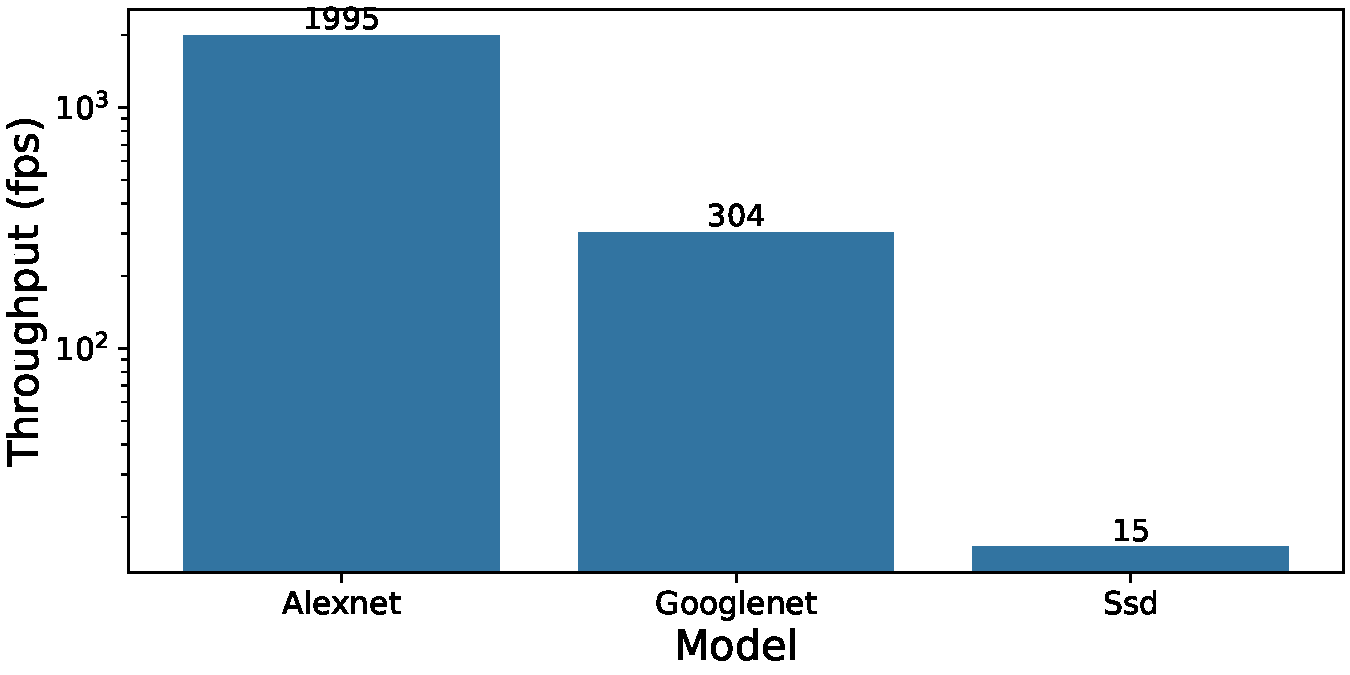
\includegraphics[width=\textwidth]{chapters/roomie/images/Throughput_models_in_isolation.pdf}
		\caption{Throughput when the model operates in isolation, without any interference.}
		\label{fig:isolation}
	\end{subfigure}
	\hfill
	\begin{subfigure}[t]{0.45\textwidth}
		\centering
		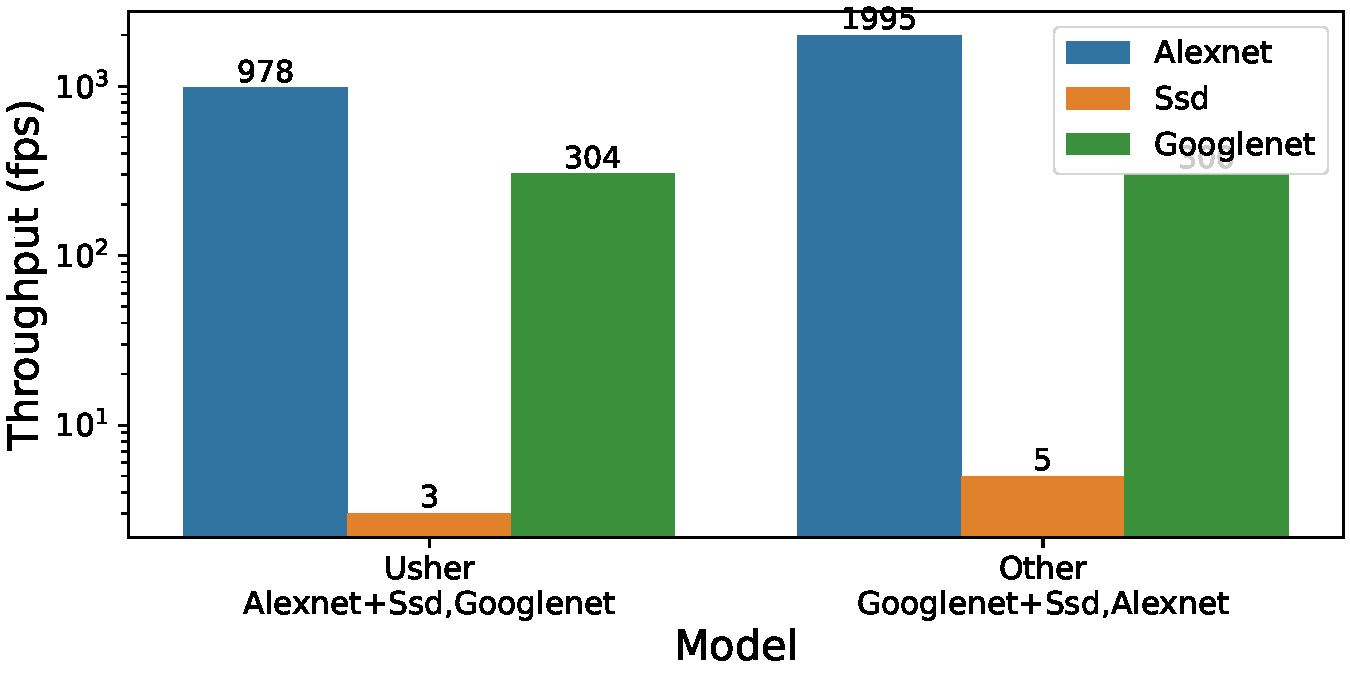
\includegraphics[width=\textwidth]{chapters/roomie/images/Throughput_models_in_combinaison.pdf}
		\caption{An alternative to co-locating three models on two GPUs, offering a better compromise than Usher~\cite{shubha2024usher}.}
		\label{fig:colocation}
	\end{subfigure}
	\label{fig:three graphs}
\end{figure}

\subsection{Limitations of Existing Inference Serving Strategies}

The deployment of machine learning models for inference serving has become increasingly critical across domains such as computer vision, natural language processing, and recommendation systems. As demand for real-time inference grows, organizations are compelled to maximize the utilization of existing computational infrastructure, particularly in resource-constrained environments. While scalable serving architectures have been proposed to meet service level objectives (SLOs), such as latency and throughput, many existing systems rely on simplistic heuristics for model placement and colocation. These approaches typically reference offline profiling data or prioritize devices with the most available memory, overlooking the nuanced performance degradation that arises when multiple models share GPU resources.

The assumption that memory availability is a reliable proxy for inference performance is mistaken. During inference, models consume significantly less memory compared to training, as intermediate states and gradients are not retained. Consequently, memory-centric placement decisions fail to account for the dynamic interference between concurrently executing models. Systems such as Usher attempt to address this by analyzing low-level GPU kernels to estimate resource demands. However, their methodology does not capture the complex interactions between kernels from different models, leading to suboptimal colocation choices.

We conducted an experimental study to evaluate the performance of three inference models: AlexNet, GoogLeNet, and SSD, on two Jetson Xavier devices. The performance of each deep neural network (DNN) when operating in isolation is illustrated in~\Cref{fig:isolation}. Our primary objective was to identify the optimal co-location configuration among all possible combinations. Our findings revealed that Usher's proposed approach of co-locating AlexNet with SSD is not necessarily the most effective option. In fact, an alternative configuration, GoogLeNet paired with SSD—demonstrates a superior balance in performance (refer to Figure colocation).

We have determined that Usher's misjudgment stems from the method used to assess model compatibility. Merely classifying models based on their computing or memory capacity does not provide a comprehensive understanding of their performance. A more nuanced approach that considers the resource demands of each model over time is essential for accurate evaluation.


\subsection{The Importance of Kernel-Level Analysis}

Deep neural networks (DNNs) perform inference by executing a sequence of GPU kernels, each responsible for specific low-level computations and defined by distinct resource requirements such as shared memory, register usage, and execution time. These kernels, rather than the high-level model architecture, constitute the true computational footprint on the GPU. Profiling tools such as Nsight Systems~\cite{nsight_systems} and Torch Profiler~\cite{torch_profiler} enable fine-grained observation of kernel behavior, revealing patterns of resource occupancy and execution timing that are often obscured at the model level. Empirical analysis shows that individual kernels frequently leave portions of the GPU underutilized, suggesting that with careful orchestration, multiple models can be deployed simultaneously to improve overall throughput.

However, when models are executed concurrently on the same GPU, their kernels may overlap in time and compete for limited hardware resources. Although this parallelism can enhance utilization, it also introduces a critical challenge: interference. This occurs when the combined resource demands of overlapping kernels exceed the GPU's capacity, forcing the hardware to serialize execution or delay kernel launches. For instance, if two kernels simultaneously require more shared memory or registers than the GPU can allocate, contention arises, leading to extended execution times and degraded performance. The severity of interference is shaped not only by the type of resources consumed but also by the duration and temporal alignment of kernel execution. Without precise modeling of these interactions, colocation decisions risk undermining system efficiency rather than enhancing it.

Effective colocation requires more than simply identifying underutilized resources; it demands a precise understanding of how kernels from different models interact during concurrent execution. The configuration of each kernel (its use of shared memory, registers, and other architectural resources) determines its potential for interference with others. Predicting these interferences cannot be based solely on aggregated model statistics or layer-level abstractions, as these overlook the fine-grained execution dynamics that govern actual performance. Instead, kernel-level analysis must consider both static resource requirements and temporal execution behavior to assess how overlapping workloads compete for limited GPU capacity. By modeling these interactions, it becomes possible to identify model pairs that minimize conflicts and make informed colocation decisions that preserve throughput and latency under constrained conditions.

\subsection{Challenges in Modeling and Predicting Interference}

% \begin{figure}
% 	\centering
% 	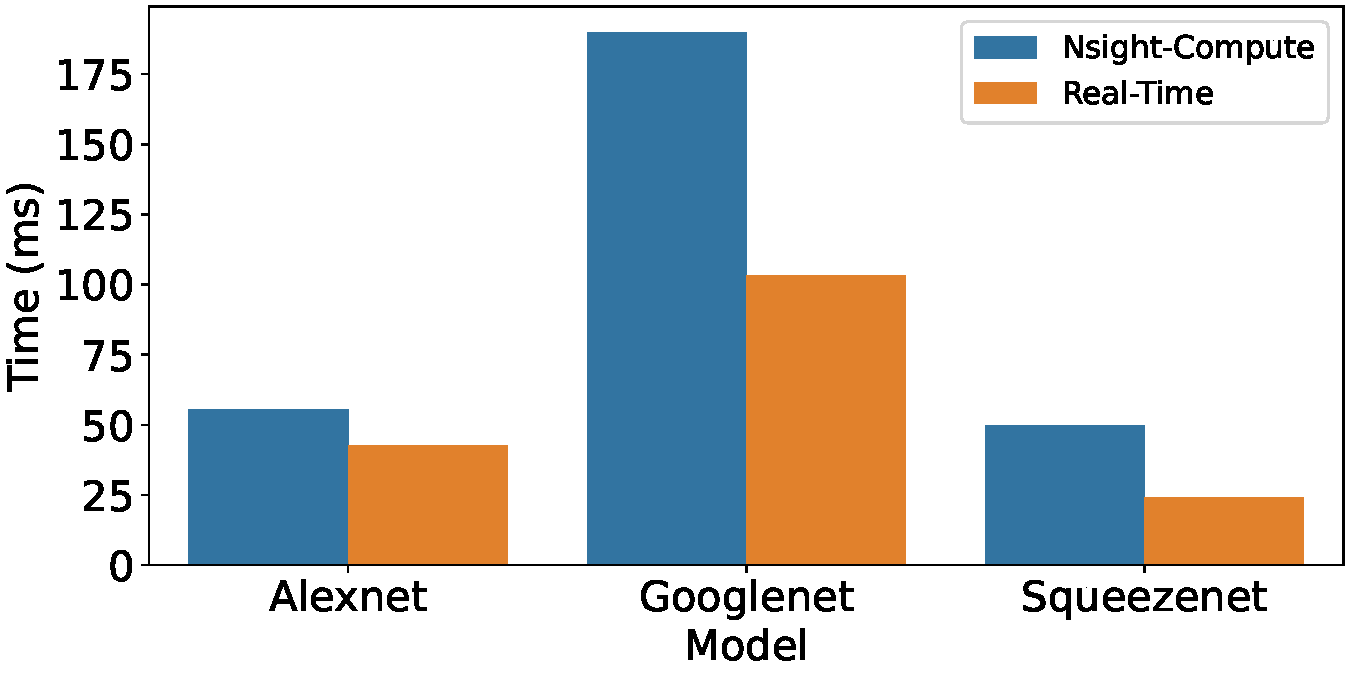
\includegraphics[width=\textwidth]{chapters/roomie/images/duration_gap.pdf}
% 	\caption{Throughput when the model operates in isolation, without any interference.}
% 	\label{fig:duration_gap}
% \end{figure}

Determining the best colocation strategy for deep neural networks (DNNs) sharing a GPU requires a nuanced understanding of how their kernels interact during inference. The goal is to identify model pairings that maximize throughput and minimize latency by avoiding harmful interference. Achieving this demands accurate performance modeling at the kernel level, where resource contention and execution overlap directly impact runtime behavior. However, building such models introduces several practical and computational challenges that must be addressed to ensure scalability and reliability.

\paragraph{Profiling overhead and trace collection.}
% Profiling is essential for capturing the fine-grained execution characteristics of DNN kernels, including resource usage and execution time. These metrics form the backbone of any interference-aware colocation strategy. Yet, collecting accurate traces is inherently time-consuming and introduces overhead that can distort the very measurements it seeks to record. Profiling tools rely on instrumentation and callbacks that add latency to kernel execution, often resulting in total recorded durations that exceed the actual inference time. This discrepancy complicates performance estimation and can mislead scheduling decisions if left uncorrected. Despite these limitations, profiling remains indispensable, as predicting kernel behavior analytically is highly challenging due to the variability in runtime configurations and hardware-specific optimizations. Fortunately, the process can be made tractable by profiling models in isolation. Since the number of GPU architectures in deployment is relatively small, and many models follow standardized execution patterns, it is feasible to build a reusable profiling database that supports accurate interference modeling without incurring prohibitive cost.
% Profiling is crucial for capturing the detailed execution characteristics of Deep Neural Network (DNN) kernels, particularly regarding resource usage and execution time, which are essential for interference-aware colocation strategies. However, the process of collecting accurate execution traces is time-consuming and introduces overhead that can distort measurements, often resulting in recorded durations that exceed actual inference times. This discrepancy complicates performance estimation and may mislead scheduling decisions if uncorrected. Despite these limitations, profiling is indispensable, as predicting kernel behavior analytically is challenging due to variability in runtime configurations and hardware-specific optimizations. Profiling models in isolation can alleviate some of these issues, and given the relatively small number of GPU architectures in use and the standardized execution patterns of many models, it is feasible to create a reusable profiling database that supports accurate interference modeling without incurring prohibitive costs.
Profiling is essential for capturing the fine-grained execution characteristics of DNN kernels, including resource occupancy and duration. These metrics form the backbone of any interference-aware colocation strategy. Yet, collecting accurate traces is inherently time-consuming and introduces overhead that can distort the very measurements it seeks to record. Profiling tools rely on instrumentation and callbacks that add latency to kernel execution, often resulting in total recorded durations that exceed the actual inference time.
In practice, we observed that the ratio between profiled kernel durations and actual inference time can vary considerably, sometimes exceeding the true runtime by a wide margin, highlighting how profiling overhead may distort performance measurements and must be carefully considered.
% This discrepancy complicates performance estimation and can mislead scheduling decisions. Figure~\ref{fig:duration_gap} illustrates this phenomenon, showing the gap between the measured inference time and the aggregate kernel durations.
Despite these limitations, profiling remains indispensable, as predicting kernel behavior analytically is highly challenging due to the variability in runtime configurations and hardware-specific optimizations. What's more, cuDNN~\cite{cudnn} provides highly tuned implementations for standard routines such as convolution, attention, matrix multiplication, pooling, and normalization. For the same operator type, it may execute different kernels depending on the GPU architecture and available resources, with varying configurations in register usage, shared memory, and execution strategy. While this process is time-consuming, it remains feasible due to the limited number of GPU variants and the ability to profile models only in isolation.

\paragraph{Combinatorial Complexity of Kernel Overlap Scenarios.}
% Another significant challenge lies in modeling the overlapping execution of kernels across multiple DNN models. While the analytical framework developed earlier enables estimation of interference effects, applying it exhaustively is computationally prohibitive. Real-world deployments do not guarantee synchronized kernel execution; instead, each model may begin inference from any point in its kernel sequence. Evaluating all possible alignments requires constructing a full Cartesian product of starting indices, resulting in exponential growth in the number of scenarios as the number of models increases. This combinatorial explosion makes real-time evaluation impractical.
A key challenge in optimizing deep neural network colocation lies in defining and identifying the interference itself. Interference is not a static property: it arises dynamically when the kernels of different models overlap during execution and compete for shared GPU resources. To determine which kernels are likely to interfere, it is necessary to analyze not only their resource requirements, but also their temporal alignment and execution context. This is particularly difficult because interference depends on both the type and timing of resource usage, which can vary across deployments and hardware configurations.\\
This challenge is compounded by the vast number of possible overlapping scenarios. In realistic service environments, models do not begin inference in a synchronized manner; each can start at any point in its kernel sequence, leading to a vast space of potential execution alignments. Taking into account all combinations of starting positions across multiple models leads to exponential growth in the number of scenarios as the number of models increases. This combinatorial explosion makes exhaustive evaluation impractical for real-time decision-making. The challenge lies in estimating the impact of interference without simulating all possible alignments, while maintaining sufficient fidelity to guide effective colocation strategies.

To support efficient colocation of deep neural networks on shared GPUs, we introduce~\roomie, a kernel-level profiling and interference estimation strategy that balances precision with scalability. By analyzing execution traces in isolation and simulating representative overlap scenarios,~\roomie{} enables informed deployment decisions without incurring prohibitive computational cost.



% Modeling kernel interference presents several challenges. First, the diversity of GPU architectures and model types necessitates extensive offline profiling to capture performance characteristics across deployment scenarios. While this process is time-consuming, it remains feasible due to the limited number of GPU variants and the ability to profile models in isolation. Second, predicting interference requires identifying which kernels will overlap in execution and assessing the impact on their runtime. This involves analyzing resource contention at a granular level, including shared memory and register usage, and determining whether the combined demand exceeds the GPU's capacity.

% Furthermore, the execution order of kernels and their serialization within CUDA streams influence the degree of interference. Kernels with complementary resource profiles may coexist with minimal performance degradation, while those with overlapping demands can significantly delay each other's execution. Existing approaches that rely solely on layer-level information or aggregate model statistics fail to capture these subtleties. Therefore, a more refined methodology is required—one that profiles kernels individually, models their interactions, and predicts the resulting performance impact under colocation. Addressing these challenges is essential for enabling efficient inference serving in environments where computational resources are limited and colocation is unavoidable.
\section{Related Work}\label{sec:related}

With the proliferation of deep learning-based applications offered as online services, managing and scheduling large-scale inference workloads in GPU data centers has become increasingly critical. Unlike resource-intensive training workloads, inference tasks have distinct characteristics that require specialized scheduling solutions. The objectives of inference scheduling (accuracy, latency, and cost-effectiveness) are closely linked. Accuracy efficiency involves selecting the most suitable model for each query and allocating resources intelligently. Latency efficiency requires meeting response time constraints, even in the face of irregular or fluctuating loads. Cost efficiency aims to minimize financial expenditure, particularly in public cloud environments. These objectives are often contradictory, requiring flexible and comprehensive planning systems capable of balancing trade-offs between different performance dimensions.

\paragraph{Inference Serving Systems.}
Several systems have been proposed to address the challenges of inference scheduling. Clipper~\cite{2017Clipper} supports multiple ML frameworks and simplifies model deployment for real-time applications, but does not account for resource interference. TensorFlow-Serving~\cite{olston2017tensorflow} adapts to traffic changes by scaling replicas, yet similarly overlooks interference among colocated models. Clockwork~\cite{gujarati2020servingDNNlikeclockwork} offers predictable performance by executing one inference at a time with full GPU capacity, but this design underutilizes GPU resources due to limited concurrency. Proteus~\cite{ahmad2024proteus} introduces adaptive batching and dynamic model variant selection to optimize throughput and accuracy. However, its restriction of one model variant per device limits co-location and parallel execution, leaving GPU resources underexploited.

\paragraph{Multi-Tenant DNN Inference on Shared GPUs.}
To improve resource utilization, recent work has explored concurrent execution of multiple models on shared GPUs. INFaaS~\cite{francisco2021infaas} enables model-less serving by dynamically selecting variants based on query load and performance constraints. It co-locates variants and scales workers reactively, but struggles with profiling complexity and lacks proactive interference prediction. Colti~\cite{mobin2023colti} enhances throughput by colocating models for training and inference. Yu et al.~\cite{yu2021automated} exploit operator-level independence to schedule concurrent execution across streams, reducing latency. REEF~\cite{han2022microsecond} supports kernel preemption and priority-based sharing to maintain predictable performance. Miriam~\cite{zhao2023miriam} introduces elastic kernels for real-time prioritization, enabling flexible scheduling across tasks with varying criticality. While these systems optimize post-deployment execution, they often neglect initial placement strategies that could preemptively mitigate interference.

\paragraph{Interference-Aware Inference Serving.}
Recent studies have focused on proactive scheduling by modeling and predicting interference between concurrently running models. Mendoza et al.~\cite{mendoza2021interference} propose a latency degradation model based on global buffer and PCIe utilization, but the coarse granularity limits predictive accuracy. Scrooge~\cite{hu2021scrooge} profiles concurrency thresholds for identical DNNs to determine optimal co-location, yet its approach is infeasible for heterogeneous model combinations due to profiling overhead. Abacus~\cite{cui2021Abacus} schedules operators from multiple models jointly to maintain QoS, but its hardware-agnostic duration model and reactive execution lead to underutilization and increased latency. iGnifer~\cite{xu2023iGniter} adopts a low-level perspective, using GPU metrics such as L2 cache usage and core launch counts to characterize interference. However, coarse indicators like power consumption prove less predictive. Usher~\cite{shubha2024usher} refines interference modeling by analyzing kernel occupancy and DRAM usage, distinguishing between compute- and memory-intensive workloads. Both Usher and iGnifer rely on NVIDIA's Multi-Process Service (MPS)~\cite{nvidiaMPS575} for spatial sharing, which limits their applicability in edge environments such as NVIDIA Jetson, where MPS is unsupported.
\section{Kernel Interference-Aware Scheduling}\label{sec:kernel_interference_aware_scheduling}
This section explains the main concept behind~\roomie. First, we introduce the idea of interference and describe a method for estimating it. Next, we present an algorithm that efficiently calculates the interference among various models. Finally, we detail a placement algorithm that utilizes the interference estimation from the first procedure to efficiently allocate new incoming models to the available GPUs.

\subsection{Kernel Interference Estimation}

% When a new request arrives, you must perform two actions: choose a variant and select the resource in which to deploy it. Several strategies can be used to choose a variant. You can choose the fastest variant for a time-constrained application, or the most accurate but potentially slower variant. This information is often obtained by profiling the model off-line.

%Kernel-level interference takes into account the interference that the kernels of several models deployed on the same GPU resource may have with each other. 
%When a model is running for inference on an NVIDIA GPU, it launches a sequence of kernels for each of its layers. A kernel represents a single operation executed by many threads in parallel. Each kernel is launched with a configuration that defines the size of the kernel grid, the division of the grid into blocks and the GPU resources required (\eg, registers per thread, shared memory per block) to execute the kernel. A grid is an array of thread blocks. % and a block represent a 1D, 2D or 3D array of threads. \ff{Not clear, what is a grid? We should be more detailed here and add more references.} 
%Threads within a block can share memory and synchronize their execution. Choosing an efficient launch configuration maximizes device utilization. A group of 32 threads within a cooperative thread arrays (CTAs) or blocks is called warps. A streaming multiprocessor (SM) handles execution of a kernel as groups warps. Blocks are the basic units of execution on the GPU and are scheduled to run on the multiprocessors of the GPU. Each block is given a certain amount of shared memory and a maximum number of threads it can contain, which is hardware-dependent.

%The execution resource demands of individual threads ultimately constrain the maximum number of threads that can be active (running) simultaneously. There are multiple hardware limitations such as the maximum number of threads per block, the maximum registers per thread, maximum registers per block, just to name some. While exceeding some of these limitations will prevent the kernel from executing like the maximum registers per thread, others prevent the kernel from using all resources that will be in its disposable. When a kernel is limited by the number of warps that can be active at the same time in a SM this is characterized as limited by warps. A kernel is limited by registers when the number of registers per thread exceed total registers available per multiprocessor. A kernel is memory limited when the amount of shared memory available per multiprocessor limits the number of blocks that can be active at the same time. 
%Many other limitations might also prevent a kernel from full using GPU resources such as memory bandwidth of the GPU necessary for transferring data GPU memory and the multiprocessors. Therefore, the occupancy is the ratio of the number of active warps per multiprocessor to the maximum number of possible active warps. The theoretical occupancy can be calculated offline and represents the upper limit of occupancy imposed by the kernel launch configuration and the capabilities of the CUDA device~\cite{lim2017autotuninggpukernelsstatic}. On the other hand, the achieved occupancy is measured during kernel execution and represent actual occupancy of the GPU.

% With that knowledge, when two kernels are executed at the same time, warp schedulers responsible for scheduling warps can schedule different warps from different kernels to run in parallel when the hardware resource allows it.

% Then kernel level interference would be the effectiveness of leveraging the insight of kernel execution and exploiting that to determine how multiple kernels might interference one other. In fact, when kernels have different limitations that can eventually lead the possible of running multiple of them at the same time. However, when kernels from different models at a specific time are requested for execution, there will be interference if on prevent another from reaching it previously preditermined occupancy. In other words, si un kernel avait au départ une certaine occupancy et que ce dernier doit partager les resources disponibles avec un autre kernel et que celui-ci reduit some nombre de block as explained previously, then this kernel will be considered in interference. And the performance drop can be computed according to the new occupancy.
% Understanding how kernels execute is crucial for recognizing how they can interfere with one another. Interference happens when one kernel prevents another from reaching its intended performance level while both are scheduled to run simultaneously. In simpler terms, interference occurs when the demand for resources from multiple kernels at the same time exceeds the total resources that the GPU can provide. If a kernel is designed to operate at a certain capacity but must share resources with another kernel, it may end up with fewer resources available for its tasks. In this case, we say the kernel is experiencing interference. This interference can lead to lower performance, which can be measured by determining the new kernel achievement, i.e., occupancy. And this new achievement can be used to determine the new execution time of the kernel, as it may take longer to complete its tasks with fewer resources. We will demonstrate that accurately estimating this interference at the kernel level is essential for effectively managing the allocation of new models on GPUs, as it allows for better resource distribution and improved overall performance.

Understanding how kernels execute is crucial for recognizing how they can interfere with one another. Interference happens when one kernel prevents another from reaching its intended performance level while both are scheduled to run simultaneously. In simpler terms, interference occurs when the demand for resources from multiple kernels at the same time exceeds the total resources that the GPU can provide. If a kernel is designed to operate at a certain capacity but must share resources with another kernel, it may end up with fewer resources available for its tasks. In this case, we say the kernel is experiencing interference.
This interference can lead to lower performance, which can be measured by determining the kernel's new achievement, specifically its occupancy. This new occupancy can then be used to estimate the kernel's execution time, as it may take longer to complete its tasks with fewer resources. We will demonstrate that accurately estimating this interference at the kernel level is essential for effectively managing the allocation of new models on GPUs, as this helps to improve overall performance.

%would be the effectiveness of exploiting knowledge of kernel execution to determine how multiple kernels can interfere with each other and how to measure the degree of interference. 

\paragraph{Model kernels.}

When a model runs inference on an NVIDIA GPU, each layer is executed by launching one or multiple kernels, a computational routine that runs in parallel across many threads. These threads are grouped into warps, typically sets of 32 threads that execute instructions in lockstep. Warps ($W$) themselves are organized into blocks ($b$), which serve as the basic scheduling units on the GPU. Blocks are assigned to streaming multiprocessors (SMs), the core computational engines that execute instructions and manage local resources such as registers and shared memory. The efficiency of each kernel depends on how it uses GPU resources, such as registers allocated per thread and shared memory available during execution. While the full execution model involves additional structural details, we focus here on threads, warps, blocks, and resource usage to highlight the core mechanisms relevant to performance. For a comprehensive description of the CUDA execution model, refer to the official documentation~\cite{nvidia2025cuda}.

From this understanding of kernel execution, we can determine its theoretical occupancy, which reflects how many warps are active relative to the hardware's capacity by the following equation :

\begin{equation}\label{eq:occupancy}
	o = \frac{W_b \times b}{W}
\end{equation}
,where $W_b$ is the number of warps per block, $b$ is the number of blocks assigned to an SM, and $W$ is the maximum number of warps the SM can support.

This value provides an overview of the number of active tasks in relation to the hardware's capacity to execute them simultaneously. It is called theoretical utilization because it represents the optimal scenario in terms of the GPU's potential workload. However, it does not guarantee that the kernel will operate efficiently. For a thorough understanding of how it is calculated, please refer to the source in~\cite{lim2017autotuninggpukernelsstatic}.

\paragraph{Kernel Interference.} We characterize a GPU by its capacity $\Phi$, which encompasses hardware limits such as the maximum number of warps, the size of the register file, and the amount of shared memory available per streaming multiprocessor (SM). These resources constrain the execution of a kernel, e.g., the maximum number of warps, the size of the register file, or the shared memory per multiprocessor~\cite{lim2017autotuninggpukernelsstatic}. For a set of kernels $K$ launched to run on the same GPU, interference occurs when the total resource demand exceeds the device's capacity. More formally,

\begin{equation}\label{eq:occurrence}
	\sum_{k \in K} \varphi_k > \Phi
\end{equation}
,where $\varphi_k$ (e.g., warps, registers, and shared memory) denotes the resource usage of kernel $k$, and $K$ is the set of active kernels.

\paragraph{Interference Modeling via Theoretical Occupancy Adjustment.} The main challenge lies in estimating the interference each kernel experiences when executed alongside others. This depends on how the theoretical occupancy is recalculated relative to the capacity of the GPU resources $\Phi$. Since GPU resources are shared among concurrent kernels, they can be redistributed in different ways, and each allocation yields a different occupancy outcome. Various strategies are possible: equal distribution, first-come-first-served, or allocation based on priorities. Each of these affects the amount of resources allocated to the kernel and its performance. Given that the available resources constrain the maximum number of blocks a kernel can launch, we can compute a new maximum blocks $\tilde{b}_k$ for each kernel $k$, based on the redistribution of the GPU resources $\Phi$. For details on this calculation, refer to~\cite{lim2017autotuninggpukernelsstatic}, or consult the implementation provided in our open-source code.

With the new block limit $\tilde{b}_k$, we can derive the new occupancy $\tilde{o}_k$ using the same formulation as in~\Cref{eq:occupancy}. This allows us to estimate the new execution time of the kernel under interference:

\begin{equation*}
	\tilde{d}_k = d_k \times \frac{o_k}{\tilde{o}_k}
\end{equation*}
, where $d_k$ is the execution time of kernel $k$ when running in isolation. Worth mentioned that, if $o_k = \tilde{o}_k$, then no interference occurs, and $\tilde{d}_k = d_k$.

% Interference ends once the first kernel completes its execution. Assuming at most two kernels are interfering, we define the interference period as the time required for the first kernel $k^*$ to finish, $\Delta = \min \left\{ \bar{d}_k \right\}_{\forall k \in K}$.

% \begin{equation*}
% 	\bar{d}^{'}_k = \left(\bar{d}_k - \Delta \right) \times \frac{\tilde{o}_k}{o_k}
% \end{equation*}

Interference ends once the first kernel completes its execution. Assuming at most two kernels are interfering, the remaining kernel continues alone without interference. We define the interference period as the time required for the first kernel to finish, $\Delta = \min \left\{ \tilde{d}_k \right\}_{\forall k \in K}$.
For the remaining kernel, its total duration is composed of two phases: the initial interference period $\Delta$, during which it runs with reduced occupancy $\tilde{o}_k$, and the remaining portion of its execution, which proceeds at full occupancy $o_k$. To account for the change in execution speed, we adjust the remaining time accordingly. Specifically, the portion $\tilde{d}_k - \Delta$, originally computed under reduced occupancy, is scaled by $\frac{\tilde{o}_k}{o_k}$ to reflect the normal execution once interference ends. Formally expressed:

\begin{equation}
	\tilde{d}_k =
	\begin{cases}
		\tilde{d}_k & \text{if } \tilde{d}_k \leq \Delta \\
		\Delta + \left( \tilde{d}_k - \Delta \right) \times \frac{\tilde{o}_k}{o_k} & \text{otherwise}
	\end{cases}
\end{equation}

% \begin{equation}
% 	\tilde{d}_k=
% 	\begin{cases}
% 		k_{i\omega}/k_{p\omega}=2\pi\times 10 \\
% 		\left\lvert\frac{k_{p\omega}s+k_{i\omega}}{s}\cdot\frac{1}{Ts+1}\right\rvert_{S=\mathrm{j}\cdot2\pi}=1
% 	\end{cases}\,.
% \end{equation}

This unified notation allows us to express the adjusted duration for all kernels, whether they complete during the interference window or continue beyond it.

\paragraph{Performance Drop.} Now that we have established a method for estimating interference among simultaneously executing kernels, we can generalize this approach to the inference phase of multiple DNNs. Each DNN launches a sequence of kernels, and we begin by aligning the first kernel of each DNN to form an initial set of concurrently executing kernels. This set is evaluated using the interference model described above. Once the first kernel in the set completes, it is replaced by the next kernel from the same DNN, and the process continues iteratively until all models have completed their execution, that is, until all final kernels have been processed.

For a model with an original inference time $T$ and a total of $q$ kernels, the new inference time under interference is given by:
\begin{equation*}
	\tilde{T} = \sum_{i=1}^{q} \tilde{d}_{k_i}
\end{equation*}

The performance drop experienced by model $m$ due to interference is quantified by the relative increase in inference time. This is computed as:
\begin{equation}\label{eq:performance_drop}
	\mu = \frac{\sum_{i=1}^{q} (\tilde{d}_{k_i} - d_{k_i})}{\sum_{i=1}^{q} d_{k_i}} = \frac{\tilde{T} - T}{T}
\end{equation}

This formulation captures the cumulative slowdown introduced by resource contention across all kernels in the model's execution pipeline.

% Performance Drop. Now that we have an idea of how we can determine interference between multiple simultaneous kernels, we can generalize this to all kernels that simultaneous DNNs launch during the inference of multiple DNNs. We could first align the kernels of each DNN and form a first set of kernels that would run simultaneously and follow the above formulation. Then, the first kernel to finish in this set would be replaced by the next kernel of the DNN to which it belongs. We continue in this manner until all models are completed, i.e., until all the last kernels are reached. After that, a model with an initial inference time $T$ and a total of $q$ kernels would have a new inference time:

% \begin{equation*}
% 	\tilde{T} = \sum^{q}_{i=1} \tilde{d}_{k_i}
% \end{equation*}

% Finally, the performance drop caused by the interferences on a given model, is given by the increase of the inference time, \ie, the sum of kernels' new durations after interference. The performance drop of the model $m$ is determined as:
% \begin{equation}\label{eq:perfDrop}
% 	\mu = \frac{\sum^{q}_{i=1} (\tilde{d}_{k_i} - d_{k_i})}{\sum^{q}_{i=1} d_{k_i}} = \frac{\tilde{T} - T}{T}.
% \end{equation}



% =========



% To estimate the interference within a group of models deployed on a GPU, we need to determine the interference between the kernels of the different models. Given the set of kernels $K_t$ at a particular time $t$ launched by each model on a GPU, the interference will consist in re-distributing the GPU resources $\Phi$ among all the different kernels in $K_t$. We represent with $\bar{\varphi}_k$ the maximum resource allocable to kernel $k \in K_t$ after the re-distribution according to one of the strategies described before.


% We denote by $M$ the set of models deployed on the GPU. Each model $m \in M$ launches a set of kernels $K_m$ for inference. Each kernel $k \in K_m$ is characterized by its duration $d_k$ (in terms of $ms$ or $ns$), its theoretical occupancy $occ_k \in \left[ 0,\, 1\right]$, and required resources $\varphi_k$ (that can be in terms of warps, registers, and shared memory). The theoretical occupancy $occ_k$ represents the highest level of GPU resource utilization that kernel $k$ can achieve during execution. It is calculated as the ratio of active warps per streaming multiprocessor (SM) to the maximum number of warps that the SM can support. Additionally, it reflects the maximum number of thread blocks that can run concurrently, which is constrained by the availability of wraps, registers, or shared memory~\cite{lim2017autotuninggpukernelsstatic}~\footnote{In our code is also available the implementation of the calculation of the theoretical GPU occupancy}. For a given kernel $k$, we represent with $b_k$ its maximum number of allocable blocks.

% The inference time for model $m$ deployed the GPU is defined as:
% \begin{equation}\label{eq:infTime}
% 	T_m= \sum_{k\in K_m} d_k
% \end{equation}
% Each model launches at most one kernel at time $t$, and we represent all kernels launched at that time by each model on the same GPU as $K_t$.

% We define the \textit{occurrence of interference} among kernels in $K_t$ when the sum of the requested resources exceeds the limits of the GPU device. More formally,
% \begin{equation}\label{eq:occurrence}
% 	\sum_{k \in K_t} \varphi_k > \Phi.
% \end{equation}

% In the event of interference, available resources are shared, leading to an increase in the execution time of kernels launched on the GPU. For the re-distribution of GPU resources to kernels in $K_t$, different strategies can be considered. For example, GPU resources can be equally distributed to all kernels in $K_t$, or each kernel can receive a potion of GPU resource proportionally to its demand. Alternatively, priorities strategies can be applied, such as First-Come First Served (FCFS), where resources are assigned to the kernel with the highest priority.

% \paragraph{Interference estimation} To estimate the interference within a group of models deployed on a GPU, we need to determine the interference between the kernels of the different models. Given the set of kernels $K_t$ at a particular time $t$ launched by each model on a GPU, the interference will consist in re-distributing the GPU resources $\Phi$ among all the different kernels in $K_t$. We represent with $\bar{\varphi}_k$ the maximum resource allocable to kernel $k \in K_t$ after the re-distribution according to one of the strategies described before.

% Starting from $\bar{\varphi}_k$, we can then determine the new maximum number of blocks denoted as $\bar{b_k}$ for each kernel $k$ in $K_t$ as defined in equation (1) of~\cite{lim2017autotuninggpukernelsstatic}.
% Given $\bar{b_k}$, we can finally determine the new GPU occupancy for $k$:
% \begin{equation}
% 	\bar{occ}_k = \frac{\mathbf{W}_{b_k} \times \bar{b}_k}{\mathbf{W}},
% \end{equation}
% where $\mathbf{W}$ represents the maximum number of active warps per multiprocessors, and $\mathbf{W}_{b_k}$ defines the number of warps that can be activated by the kernel during its execution.
% With this we can determine the interference time, which we consider to be the time needed for the first $k^*$ kernel to complete its execution. This time is called $\Delta$ and is defined as the minimum from all kernel execution times.
% \begin{equation}
% 	\Delta = \min \left\{ d_k \times \frac{occ_k}{\bar{occ}_k} \right\}_{\forall k \in K_t}.
% \end{equation}
% Finally, we can determine the additional time or remaining time to compute for each kernel, noted $d'$, as such:
% \begin{equation}
% 	d_k' = d_k - \Delta \times \left(1 - \frac{\bar{occ}_k}{occ_k} \right) ,\, \forall k \in K_t.
% \end{equation}

% Thus, the total duration for each kernel, given the interference, is
% \begin{equation}
% 	D_k = d_k' + \Delta.
% \end{equation}

% \paragraph{Performance Drop}
% Once a model $m$ has executed all its kernels, it concludes a full round and the new inference time is given by:
% \begin{equation}
% 	\bar{T_m} = \sum_{k \in K_m} D_k
% \end{equation}

% Finally, the performance drop caused by the interference, is given by the increase of the inference time, \ie, the sum of kernels' new durations after interference. The performance drop of the model $m$ is determined as:
% \begin{equation}\label{eq:perfDrop}
% 	\mu_m = \frac{\sum_{k\in K_m}(D_k-d_k)}{\sum_{k\in K_m}d_k} = \frac{\bar{T}_m - T_m}{T_m}.
% \end{equation}

% \subsection{Greedy Algorithm for Model interference}

\subsection{Greedy Algorithm for Estimating Model Interference}

The analytical framework developed above provides a way to estimate performance degradation due to kernel interference across multiple deep neural networks (DNNs) sharing a GPU. However, applying this model exhaustively, by evaluating all possible combinations of kernel alignments across models, is computationally infeasible. For instance, while our previous formulation assumed that all models begin execution with their first kernel simultaneously, a more general scenario would allow each DNN to start from any of its $i$-th kernels (where $1 \leq i \leq q$). Enumerating all such combinations would require constructing a full Cartesian product of starting indices, which leads to exponential growth in the search space. For $N$ concurrent DNNs, this results in a combinatorial explosion, making real-time evaluation impractical.

To address this, we propose a heuristic algorithm that approximates the interference impact efficiently. The pseudocode is presented in Algorithm~\cref{algo:kernel_interference_algorithm}. The key idea is to reduce the search space by:

1. Limiting the number of starting points per model to a subset of $n$ evenly spaced indices from the full set of $q$ kernels.
2. Focusing on \textit{pairwise interference} rather than evaluating all $N$-way combinations.

For each model pair $(m_i, m_j)$, we define a reduced set of starting indices $S_i$ and $S_j$, and construct the set of concurrent execution scenarios as:

\begin{equation*}
	\mathcal{C}_{i,j} = S_i \times S_j, \quad \text{where } S_i = \{0, n, 2n, \dots, (p_i - 1)n\}
\end{equation*}

Each scenario corresponds to a pair of starting indices $(s_i, s_j)$, which determine the positions in the kernel sequences where concurrent execution begins (line 8 in~\Cref{algo:kernel_interference_algorithm}). These serve as the basis for simulating localized interference effects between the two models.

This greedy, pairwise strategy dramatically reduces computational overhead while preserving the fidelity needed to estimate performance degradation due to kernel interference.

\paragraph{Interference Simulation.} For each pair $(m_i, m_j)$, $i \neq j$, and each starting index pair $c_{i,j}=(s_i, s_j)$, we simulate kernel-by-kernel execution. We approximate the occurrence of interference with the following new condition:
\begin{equation}
	\varphi_{k_i} + \varphi_{k_j} > \Phi
\end{equation}
In such cases, the delay added to $k_{s_i}$ (i.e., the kernel identified by the starting point $s_i$) is:

$$
	\delta_{k_{s_i}} = d_{k_{s_i}} \cdot \frac{occ_{k_{s_i}}}{occ_{k_{s_i}} + occ_{k_{s_j}}}
$$

The total delay (additional time) for a given starting pair is:

$$
	\Delta^{c_{i,j}} = \sum_{ s_i \leq t \leq q_i} \delta_{k_t}
$$

We can define the representative additional duration as the median:

$$
	\Delta_{i,j} = \text{median}\left(\left\{ \Delta^{c_{i,j}} \right\}_{\forall c_{i,j} \in \mathcal{C}_{i,j}}\right)
$$

To account for the amount of time two models interact during execution, we introduce a scaling factor that reflects their relative kernel sequence lengths:

$$
	\gamma_{i,j} = \max\left(\frac{q_i}{q_j}, 1\right)
$$

\paragraph{Determine the new duration} The new duration after interference of model $m_i$ is:

$$
	\tilde{T_{m_i}} = T_{m_i} + \sum_{\substack{j=1 \\ j \neq i}}^{N} \gamma_{i,j} \cdot \Delta_{i,j}
$$

Finally, the performance drop can be determined as defined in~\Cref{eq:performance_drop}.



% Pair-interference and Starting Combinations.


% Identifying the group of models (and hence, kernels) causing that interference is not trivial. To identify such a group, we would need to explore all possible combinations of kernels for all deployed models and verify whether the interference originates from that specific combination. This exploration is not feasible given the combinatorial explosion of the solution space. For this reason, we propose an efficient heuristic that estimates the inference among the kernels of the models deployed on the GPU. The heuristic simulates a set of possible starting points for the interference and limits the solution space to all pairs of starting points of the kernel sequences of every pair of models. In this way, we prove that considering even just an approximation of interference improves the placement of new arriving models that should be deployed on the GPU.

% To simulate concurrent execution scenarios, each model's kernel sequence is partitioned into fixed-size segments. This allows us to define multiple hypothetical starting points from which interference may begin.
% By generating all combinations of such starting indices across models, we construct a grid of scenarios that reflect different temporal alignments of kernels. These combinations serve as proxies for real-world scheduling offsets, enabling us to explore how interference might evolve depending on when models enter the execution pipeline. More formally, to simulate interference, each kernel sequence is partitioned into segments of size $n$, i.e., $p_i = \left\lfloor \frac{q_i}{n} \right\rfloor$ (line 2 in Algorithm~\cref{algo:kernel_interference_algorithm}). In this way for $n>1$, the combination space is always reduced. Furthermore, rather than constructing the full Cartesian product of starting indices among all models, we adopt a pairwise strategy. For each model pair $(m_i,m_j)$, we generate combinations from their respective sets of starting indices:
% \begin{equation}
% 	\mathcal{C}_{i,j} = S_i \times S_j, \quad \text{where } S_i = \{0, n, 2n, \dots, (p_i - 1)n\}
% \end{equation}
% This approach significantly reduces computational overhead while preserving the ability to capture localized interference effects between models.

% Each scenario is defined by a pair of starting indices $(s_i, s_j)$, selected from the sets $S_i$ and $S_j$ (line 8 in~\Cref{algo:kernel_interference_algorithm}). These indices specify the positions in each kernel sequence where concurrent execution begins, forming the basis for simulating interference between the two models.

% \paragraph{Interference Simulation.} For each pair $(m_i, m_j)$, $i \neq j$, and each starting index pair $c_{i,j}=(s_i, s_j)$, we simulate kernel-by-kernel execution. We approximate the occurrence of interference with the following new condition:
% \begin{equation}
% 	occ_{k_i} + occ_{k_j} > 1.
% \end{equation}
% In such cases, the delay added to $k_{s_i}$ (i.e., the kernel identified by the starting point $s_i$) is:

% $$
% 	\delta_{k_{s_i}} = d_{k_{s_i}} \cdot \frac{occ_{k_{s_i}}}{occ_{k_{s_i}} + occ_{k_{s_j}}}
% $$

% The total delay (additional time) for a given starting pair is:

% $$
% 	\Delta^{c_{i,j}} = \sum_{ s_i \leq t \leq q_i} \delta_{k_t}
% $$

% We can define the representative additional duration as the median:

% $$
% 	\Delta_{i,j} = \text{median}\left(\left\{ \Delta^{c_{i,j}} \right\}_{\forall c_{i,j} \in \mathcal{C}_{i,j}}\right)
% $$

% To account for the amount of time two models interact during execution, we introduce a scaling factor that reflects their relative kernel sequence lengths:

% $$
% 	\gamma_{i,j} = \max\left(\frac{q_i}{q_j}, 1\right)
% $$

% \paragraph{Determine the new duration} The new duration after interference of model $m_i$ is:

% $$
% 	\bar{T_{m_i}} = T_{m_i} + \sum_{\substack{j=1 \\ j \neq i}}^{N} \gamma_{i,j} \cdot \Delta_{i,j}
% $$

% Finally, the performance drop can be determined as defined in~\Cref{eq:perfDrop}.

%%%%%%%%%%%%%%%%%%%%%%%%%%%%%%%%

% \subsection{Greedy Algorithm for Model interference and Model Placement}

% Executing the model interference as described above takes times and increases with respect to the number of models to interfere. We have developed a heuristic version to replace our interference algorithm. As an example, we consider a sequence of kernel durations, denoted $d = (d_{k_1}, d_{k_2}, \ldots, d_{k_q}) \in \mathbb{R}^q$, corresponding to a total of $q$ kernels associated with a specific model $m$. The interference mask would be a sliding window mask applied to that vector, where the window size $w$ varies from $\frac{q}{2}$ to $q$. This denotes the window size, corresponding to the number of kernels scheduled for execution that overlap or eventually interfere with those of another model. The masking operation is applied symmetrically from both the beginning and the end of the vector, thereby capturing interference with the first and last $w$ kernels of the model, respectively.

% Let's define the forward mask (beginning) $X^{(f)}_w \in \mathbb{R}^q$ and $w \in \left[ \left\lfloor \frac{q}{2} \right\rfloor ,\, q \right]$ as:

% \begin{equation*}
% 	X^{(f)}_w[i] =
% 	\begin{cases}
% 		0       & \text{if}~i < q-w \\
% 		d_{k_i} & \text{otherwise}
% 	\end{cases}
% 	~\text{for}~i=0,\,1,\,\dots,\,q-1
% \end{equation*}

% This creates for each window of size $w$, zeroing out elements after which represent kernels that will not interfere.

% For the backward mask $X^{(b)}_w \in \mathbb{R}^q$, and $w \in \left[ q - 1 ,\, \left\lfloor \frac{q}{2} \right\rfloor - 1 \right]$ it would be:

% \begin{equation*}
% 	X^{(b)}_w[i] =
% 	\begin{cases}
% 		0       & \text{if}~i > w  \\
% 		d_{k_i} & \text{otherwise}
% 	\end{cases}
% 	~\text{for}~i=0,1,\dots,q-1
% \end{equation*}

% This creates a window of size $w$, zeroing out elements before which are considered terminated before interference.

% Finally, the full interference mask $X$, combining all forward and backward masks:

% \begin{equation}
% 	X =
% 	\begin{bmatrix}
% 		X^{(f)}_{\left\lfloor \frac{q}{2} \right\rfloor}     \\
% 		X^{(f)}_{\left\lfloor \frac{q}{2} \right\rfloor + 1} \\
% 		\vdots                                               \\
% 		X^{(f)}_{q}                                          \\
% 		X^{(b)}_{q - 1}                                      \\
% 		X^{(b)}_{q - 2}                                      \\
% 		\vdots                                               \\
% 		X^{(b)}_{\left\lfloor \frac{q}{2} \right\rfloor - 1}
% 	\end{bmatrix}
% \end{equation}

% Each row of the matrix, \ie, $X_w$, is a masked version of $d$, with zeros outside the sliding window.

% Besides the interference mask, we also define a binary probability matrix $P$ with the same size as the matrix interference. That probability stands for each kernel the probability it interferes with full resource utilization, i.e., preventing any other kernel from running with another kernel. This also means that its duration will be added to the other model inference duration.\\
% By performing an element-wise product of the two matrix $X$ and $P$ we then got the on each row the additional duration that would be added to the initial duration of any other model it interferes with. We can then use the median of each row


\begin{algorithm}[t]
	\caption{Greedy Estimation of Model Interference}
	\label{algo:kernel_interference_algorithm}
	\SetAlgoLined
	\SetKwProg{Fn}{Function}{}{end} % Function name(args) [...] end
	\Fn{performance\_drop($M$)}
	{
		\begin{small}
			Generate starting index $S_i$ for each model as Cartesian product of starting indices across all models.

			Initialize performance drop $\mu \gets []$

			\ForEach{model $m_i \in M$}{
				Initialize $\tilde{T_{m_i}} \gets \sum d_k$

				\ForEach{model $m_j$ where $j \neq i$}{
					Initialize delay set $\mathcal{D}_{i,j} \gets []$

					\ForEach{pair $(s_i, s_j) \in S_i \times S_j$}{
						$k_i \gets s_i$, $k_j \gets s_j$, $\delta \gets 0$

						\While{$k_i < q_i$ and $k_j < q_j$}{
							\If{$\varphi_{k_i} + \varphi_{k_j} > \Phi$}{
								Compute additional duration: $\delta \gets \delta + d_{i,k_i} \cdot \frac{occ_{i,k_i}}{occ_{i,k_i} + occ_{j,k_j}}$
							}
							Increment $k_i$, $k_j$
						}
						Append $\delta$ to $\mathcal{D}_{i,j}$
					}
					Compute overlap factor $\gamma_{i,j} \gets \max\left(\frac{q_i}{q_j}, 1\right)$

					Update $\tilde{T_{m_i}} \gets \tilde{T_{m_i}} + \gamma_{i,j} \cdot \text{median}(\mathcal{D}_{i,j})$
				}
				Finally, the performance drop.

				$\mu_{m_i} \gets \frac{\tilde{T}_m - T_m}{\tilde{T}_m}$

				Append $\mu_{m_i}$ to $\mu$
			}
			\Return{$\mu$}
		\end{small}
	}
\end{algorithm}


\subsection{Placement Algorithm}

The performance drop resulting from GPU resource sharing can be exploited to efficiently place new arriving models after deployment query for a new model variant or in case of upscaling meet the workload demand.
%With the biggest part now completed which is a way to determine performance drop of model that will be sharing the same GPU resource. By leveraging from that, we can determine the best colocation strategy when it comes to perform a placement whether when a new query arrives and requires a deployment of a new variant or when upscaling is needed to meet query workload demand. 
When a new model arrives, the objective is to place it in a GPU $g$ so that the average performance drop, denoted by $\bar{\mu}^g$, of all running models and the incoming model is minimal. \Cref{algo:model_placement} describes the proposed procedure to place a new model that needs to be deployed. When a new model $m_{arr}$ arrives, \Cref{algo:kernel_interference_algorithm} is applied sequentially to each GPU $g$ (line 4). The algorithm monitors the average performance drop across all deployed models to ensure it does not exceed an acceptable value, $\lambda$, which serves as a tunable parameter. The value of this parameter is chosen to ensure that the arriving model will not cause a significant performance drop in the already running models. Among all the candidate GPUs that satisfy the constraint $\bar{\mu}^g < \lambda$ (lines 7--9), the one that offers the lowest average performance drop is selected as the final deployment target. It is worth noting that this algorithm can be easily adapted to other objectives, e.g., selecting the GPU that offers the highest throughput or lowest latency. If no suitable GPU is identified, the deployment is deferred.

%the highest throughput (or shortest latency, etc.), while maintaining an acceptable performance degradation for model $m_{arr}$, is selected as the optimal deployment target. If no suitable GPU is identified, deployment is deferred.\ff{This does not seem to reflect what is written in the pseudocode. From the last two lines of \Cref{algo:model_placement} it seems that it always selects the GPU with the minimum average performance drop.}

%the algorithm (1) determines which one offers the highest throughput relative to the calculated performance drop, $\mu_{m_{arr}}$, (2) or selects the one that offers the lowest average performance drop. If such a GPU is found, it is returned as the best choice for deployment with minimal performance drop; otherwise, the deployment (or scaling) fails. \ff{This does not seem to reflect what is written in the pseudocode. From the last two lines of \Cref{algo:model_placement} it seems that it always selects the GPU with the minimum average performance drop.}

%Among the candidate GPUs that satisfy the constraint $\mu < \lambda$, the one that offers the highest throughput (or shortest latency, etc.), while maintaining an acceptable performance degradation for model $m_{arr}$, is selected as the optimal deployment target. If no suitable GPU is identified, deployment is deferred.

%This heuristic is faster and takes into account the diversity of GPUs, as models perform differently depending on the GPU hardware used, which influences interference.
\begin{algorithm}[t]
	\caption{Model Placement Algorithm}
	\label{algo:model_placement}
	\SetAlgoLined
	\SetKwProg{Fn}{Function}{}{end} % Function name(args) [...] end
	\Fn{schedule($m_{arr}, G, \lambda$)}
	{
		\begin{small}
			Initialize $p \gets []$ be sequence of performance drops of new model $m_{arr}$.

			Initialize performance drop $\mathcal{P} \gets []$
			% Initialize $s \in \mathbb{R}^p$ be sequence of performance drops of new model $m_{arr}$.

			\ForEach{ GPU $g$ }{
			$M^g \gets M^g \cup \{m_{arr}\}$

			$\mathbf{\mu}^g \gets performance\_drop($M$)$

			\tcc{Ensure no variant has a performance drop beyond $\lambda$.}

			\If{ $\bar{\mu^g} < \lambda$ }{
			Append $\mu^g_{m_{arr}}$ to $p$

			Append $\mathbf{\mu}^g$ to $\mathcal{P}$
			}
			}

			%1. Peak highest throughput.

			%$g* \gets \max \left\{ thr_{m_{arr}} - thr_{m_{arr}} * \mu^{g}_{m_{arr}} \right\}_{\forall \mu^g_{m_{arr}} \in p}$

			Peak lowest average performance drop.

			$g* \gets \min \left\{ \bar{\mu}^g \right\}_{\forall \mathbf{\mu}^g \in \mathcal{P}}$

			\Return{$g^*$}
		\end{small}
	}
\end{algorithm}



% With the biggest part now completed which is a way to determine performance drop of model that will be sharing the same GPU resource. By leveraging from that, we can deter- mine the best colocation strategy when it comes to perform a placement whether when a new query arrives and requires a deployment of a new variant or when upscaling is needed to meet query workload demand. When a new model arrives, the aim is to place it in a GPU device $g$ so that the average of the performance drops, denoted by 𝜇, of all running and the incoming model is minimal. The Algorithm 2 give a glimpse about the placement algorithm employs when a new model requires to be deployed. When a want to deploy a new model $m_{arr}$ we perform the interference algorithm (algorithm 1) sequentially on each GPU $g$ ∈ 𝐺. We use average performance drop of all models and make sure that it is not greater than an accepted value 𝜆 as a tunable parameter. This value is chosen to ensure that the arrival model won't cause important performance drop on the already running models. For the GPUs candidates, we then determine the one that gives the highest throughput with respected to computed performance drop, 𝜇, of the arriving model $m_{arr}$. If a such a GPU is found with it return as the best choice for deployment with little performance drop, otherwise nothing is return.

%When a new model arrives, the objective is to assign it to a GPU device $g$ in such a way as to minimize the average performance degradation, denoted $\mu$, across all models. The~\Cref{algo:model_placement} describes the placement procedure used when deploying a new model. More specifically, when deploying a new model $m_{arr}$, the interference evaluation algorithm (\Cref{algo:kernel_interference_algorithm}) is executed sequentially on each GPU $g \in G$. The resulting average performance degradation is then compared to a predefined threshold $\lambda$, which serves as a tunable parameter to ensure that the introduction of model $m_{arr}$ does not significantly alter the performance of existing models.

%Among the candidate GPUs that satisfy the constraint $\mu < \lambda$, the one that offers the highest throughput (or shortest latency, etc.), while maintaining an acceptable performance degradation for model $m_{arr}$, is selected as the optimal deployment target. If no suitable GPU is identified, deployment is deferred.
\section{Evaluation}

\subsection{Experimental Setup}
\label{sec:setup}


\paragraph{Baselines.} We evaluate \roomie{} against two different state-of-the-art baselines: INFaaS and Usher. INFaaS performs accuracy scaling by scaling variants within the same worker to meet demand. Usher, on the other hand, groups compute-heavy models with memory-heavy models within a group. We have used different models from two family groups, namely classification and detection, to evaluate our solution and baselines. We consider that each incoming query is intended for a single inference model.

\paragraph{Deployment Infrastructure.} We conducted our experiments using two distinct deployment types: a cluster of Jetson Nanos and a cluster of larger \acrshort{gpu}s. The first consisted of $3\times$ machines equipped with $4\times$ Nvidia \textit{A100-SXM4-40GB (40 GiB)}. The second consisted of $12\times$ Nvidia Jetson AGX Xavier \acrshort{gpu}s. Each \acrshort{gpu} is assigned to a docker to form a server, making a total of 12 servers for each deployment. We also used $2\times$ HPE Proliant DL360 Gen10+ the client requesting the model and a controller responsible for serving requests to workers. The full specifications are presented in \Cref{tab:serve_config}.

\begin{table}
	\centering
	\begin{tabular}{p{2cm}p{3cm}p{3cm}}
		\toprule
		\textbf{Model}            & \textbf{CPU}                                & \textbf{\acrshort{gpu}}                                                 \\
		\toprule

		Nvidia Jetson AGX Xavier  & 1 CPU/node, 8 cores/CPU                     & Nvidia AGX Xavier, CC~\footnote{CC: Compute capability}: 7.2 \\

		\midrule

		HPE Proliant DL360 Gen10+ & x86\_64, 2.40GHz, 2 CPUs/node, 16 cores/CPU &                                                              \\

		\midrule

		Apollo 6500 Gen10+        & x86\_64, 1 CPU/node, 32 cores/CPU           & $4\times$ Nvidia A100-SXM4-40GB (40 GiB), CC: 8.0            \\

		\midrule

		DL360 Gen10+              & x86\_64, 2.60GHz, 2 CPUs/node, 32 cores/CPU &                                                              \\

		\bottomrule
	\end{tabular}
	\caption{Server configuration used for experiments.}
	\label{tab:serve_config}
\end{table}

\paragraph{Datasets.} We evaluated our system and baseline methods using both synthetic and real-world workloads. For the real workload, we adopt the Twitter trace 2020 dataset~\cite{twitterStreamTrace2020}, as it is particularly suitable for modeling inference services, as tweets are commonly subjected to~\acrfull{dnn} processing before publication~\cite{francisco2021infaas,ahmad2024proteus}. Since the trace is aggregated at a coarse temporal granularity of one second, we apply a Poisson process to model intra-second arrival times and use a Zipf distribution to distribute queries among models, in line with established methodology~\cite{francisco2021infaas,ahmad2024proteus}.
For synthetic workloads, we generated average request rates per second using a Gaussian process and applied the same Zipf-based model allocation. To ensure our evaluation captures a broad spectrum of inference behavior, we selected a diverse and representative set of~\acrshort{dnn} models. These include both high-performance classification architectures and widely adopted object detection frameworks, enabling us to rigorously assess system behavior under varied computational and latency profiles. The full list of models is summarized in~\Cref{tab:dnn-models}, reflecting the breadth and relevance of our evaluation design.

\begin{table}[h]
	\centering \caption{Categorization of \acrlong{dnn} Models Used in Evaluation} \label{tab:dnn-models}
	\begin{tabular}{p{4cm}p{6cm}}
		\hline
		\textbf{Category} & \textbf{Models}
		\\ \hline
		Classification Models &
		\texttt{vgg19},
		\texttt{alexnet},
		\texttt{maxvit\_t},
		\texttt{resnet152},
		\texttt{googlenet},
		\texttt{densenet201},
		\texttt{squeezenet1\_1},
		\texttt{mobilenet\_v3\_large},
		\texttt{shufflenet\_v2\_x2\_0},
		\texttt{inception\_v3},
		\texttt{wide\_resnet101\_2},
		\texttt{resnext101\_32x8d},
		\texttt{efficientnet\_v2\_l},
		\texttt{convnext\_large}
		\\ \hline
		Object Detection Models &
		\texttt{ssd300\_vgg16},
		\texttt{fcos\_resnet50\_fpn},
		\texttt{retinanet\_resnet50\_fpn\_v2},
		\texttt{fasterrcnn\_resnet50\_fpn\_v2},
		\texttt{ssdlite320\_mobilenet\_v3\_large}
		\\ \hline 
	\end{tabular}
\end{table}

\paragraph{Evaluation Metrics.} To evaluate the effectiveness of each \acrshort{dnn} deployment strategy, the assessment focused on four key performance indicators. Response time measured how quickly the models delivered results, which is a critical indicator of real-time performance. The processing rate indicated the percentage of requests successfully processed, highlighting the reliability of the system for different workloads. Throughput measured the number of requests processed in a given time frame, providing insight into overall capacity and scalability. Finally, \acrshort{gpu} utilization monitored the degree of hardware resource usage during model execution.


\subsection{Performance Evaluation of Cloud-Based \acrshort{gpu} Cluster Solutions}

To assess the effectiveness of our proposed deployment strategy, we conducted a comprehensive evaluation using a cloud-based \acrshort{gpu} cluster comprising 12$\times$ \acrshort{gpu}s and all~\acrshort{dnn} models detailed in~\Cref{tab:dnn-models}. The experiments were performed using two distinct datasets: real-world Twitter data and synthetically generated data. These synthetic workloads were constructed to mimic real-world traffic patterns while allowing precise manipulation of query rates. This enabled a more granular analysis of system behavior under stress. These datasets were used to simulate varying workload intensities, beginning with low traffic levels that all models could handle and gradually increasing until system saturation was observed.

\paragraph{Evaluation on Twitter dataset.}

\begin{figure}[h!]
	\centering
	\begin{subfigure}[b]{0.45\textwidth}
		\centering
		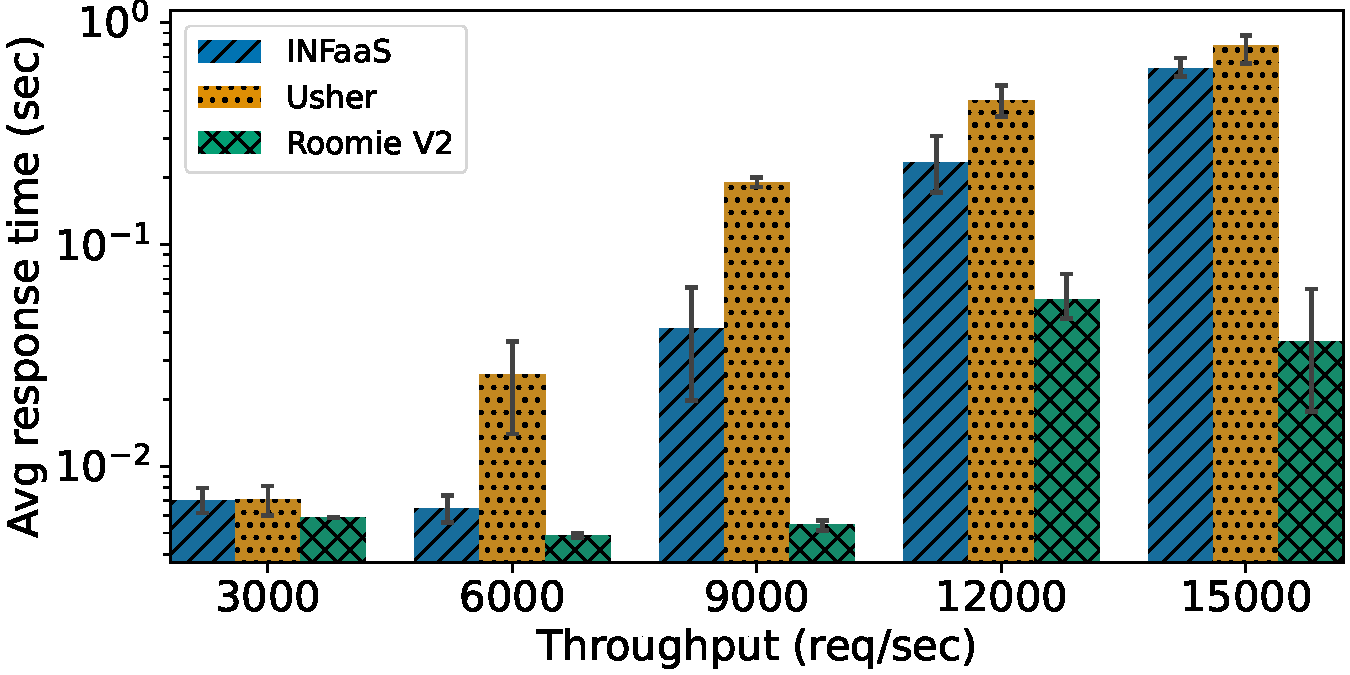
\includegraphics[width=\textwidth]{chapters/roomie/images/NvidiaA100/twitter-all-models/response_time.pdf}
		\subcaption{Response time.}
	\end{subfigure}
	\hfill
	\begin{subfigure}[b]{0.45\textwidth}
		\centering
		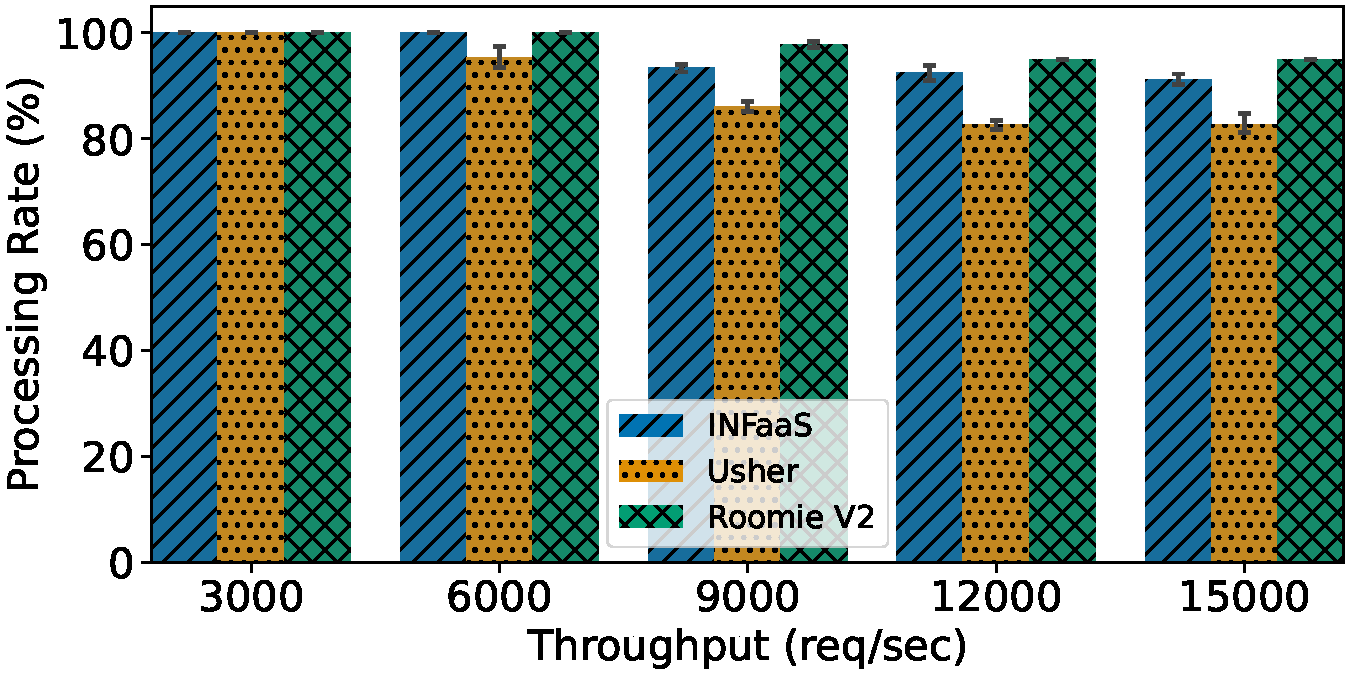
\includegraphics[width=\textwidth]{chapters/roomie/images/NvidiaA100/twitter-all-models/normalized.pdf}
		\subcaption{Processing rate.}
	\end{subfigure}
	
	\vspace{0.5cm} % Space between the rows
	
	\begin{subfigure}[b]{0.45\textwidth}
		\centering
		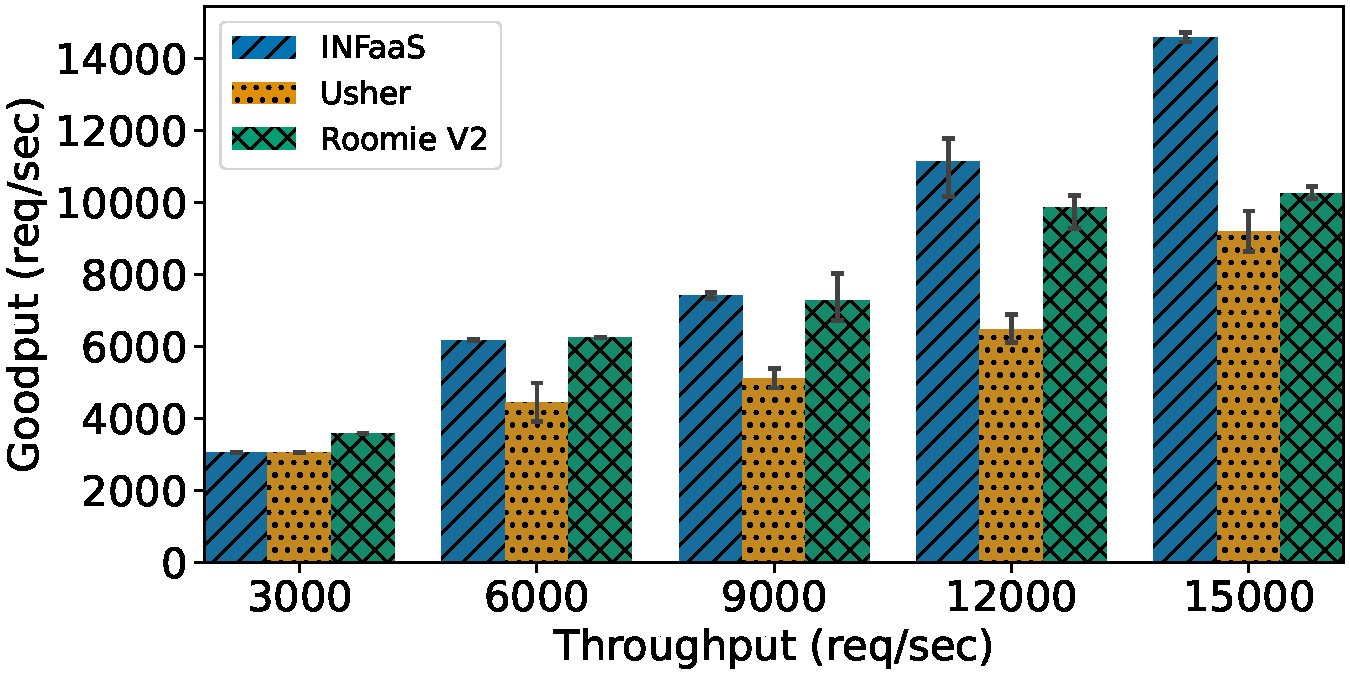
\includegraphics[width=\textwidth]{chapters/roomie/images/NvidiaA100/twitter-all-models/goodput.pdf}
		\subcaption{Goodput.}
	\end{subfigure}
	\hfill
	\begin{subfigure}[b]{0.45\textwidth}
		\centering
		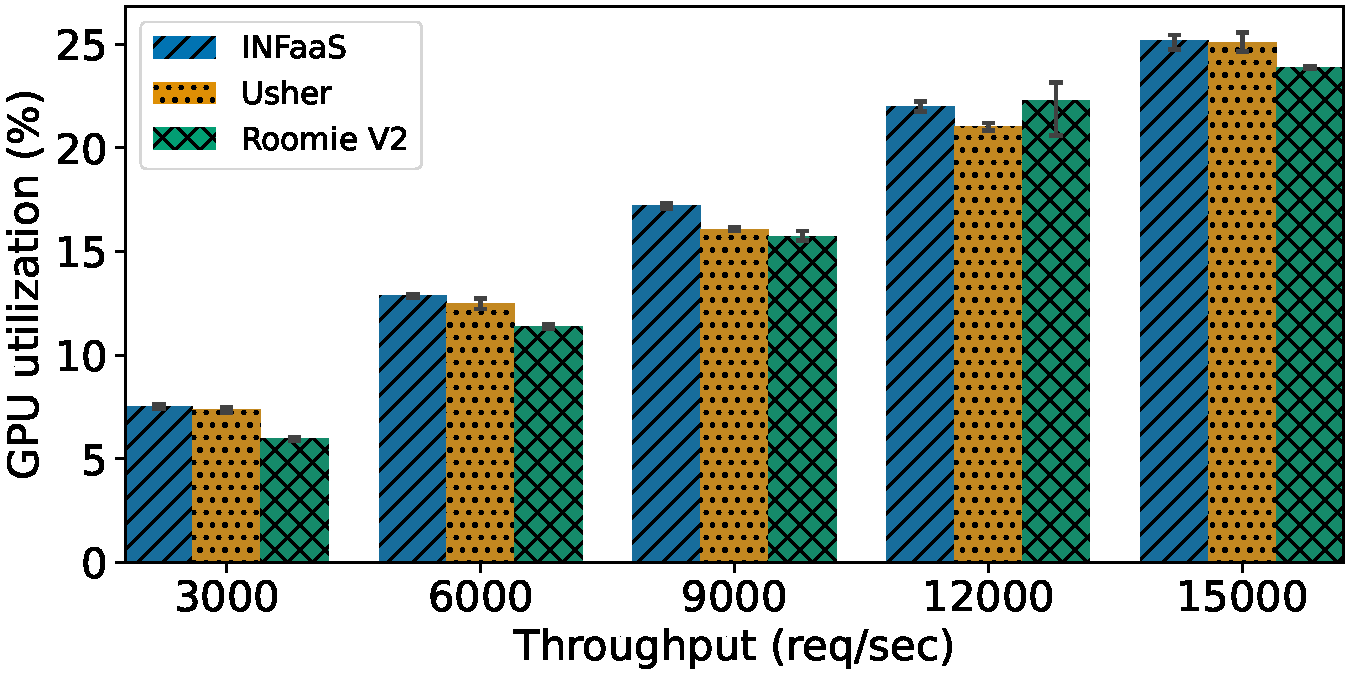
\includegraphics[width=\textwidth]{chapters/roomie/images/NvidiaA100/twitter-all-models/gpu_utilization.pdf}
		\subcaption{\acrshort{gpu} utilization}
	\end{subfigure}
	
	\caption{\roomie{} achieves up to 17$\times$ faster response times while delivering similar processing rates in a cloud-based evaluation using the Twitter dataset, outperforming INFaaS and Usher under high workload conditions.}
	\label{fig:NvidiaA100/twitter-all-models}
\end{figure}


\Cref{fig:NvidiaA100/twitter-all-models} shows the performance results obtained from the Twitter database. Under low workload conditions, all approaches showed comparable response times. However, as the workload increased, significant performance disparities emerged. Notably,~\roomie{} achieved response times up to 17× faster than rival solutions and maintained a processing rate above 97\%. In contrast, Usher's strategy of co-locating large models with lightweight models failed to deliver satisfactory performance under high load, resulting in increased latency and reduced goodput. INFaaS, which scales \acrshort{dnn}s on workers already hosting a copy, showed moderate goodput performance. However, this approach is agnostic to model interference, leading to latency increases of up to 17× and a decline in processing rate.

Interestingly, despite low \acrshort{gpu} utilization across all approaches, we observe a significant increase in response time as workload intensifies. This counterintuitive behavior can be attributed to the saturation of large models, which become unable to keep pace with incoming queries. As these models reach their computational limits, they begin to queue requests, leading to latency explosions—even though the \acrshort{gpu} itself remains underutilized. Additionally, interference between co-located models can further degrade responsiveness, compounding delays without a corresponding rise in \acrshort{gpu} activity. One potential mitigation strategy is to increase batch sizes, which can improve utilization by amortizing overhead across multiple queries. However, this approach introduces a trade-off: larger batches may inflate response times, making it unsuitable for latency-sensitive applications. These findings underscore the need for deployment strategies that go beyond raw utilization metrics and account for model saturation dynamics and cross-model interference.


\paragraph{Evaluation on synthetic dataset.}

\begin{figure}[h!]
	\centering
	\begin{subfigure}[b]{0.45\textwidth}
		\centering
		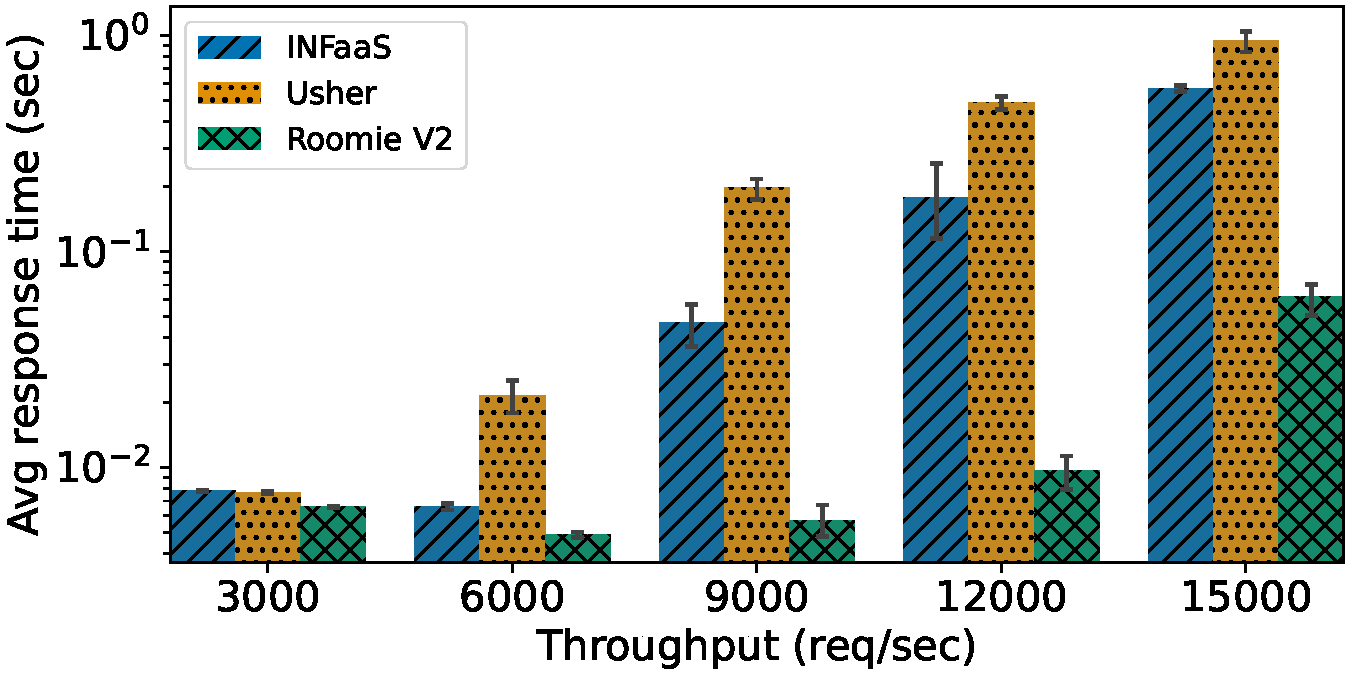
\includegraphics[width=\textwidth]{chapters/roomie/images/NvidiaA100/synthetic-all-models/response_time.pdf}
		\subcaption{Response time.}
		\label{fig:NvidiaA100/synthetic-all-models/response-time}
	\end{subfigure}
	\hfill
	\begin{subfigure}[b]{0.45\textwidth}
		\centering
		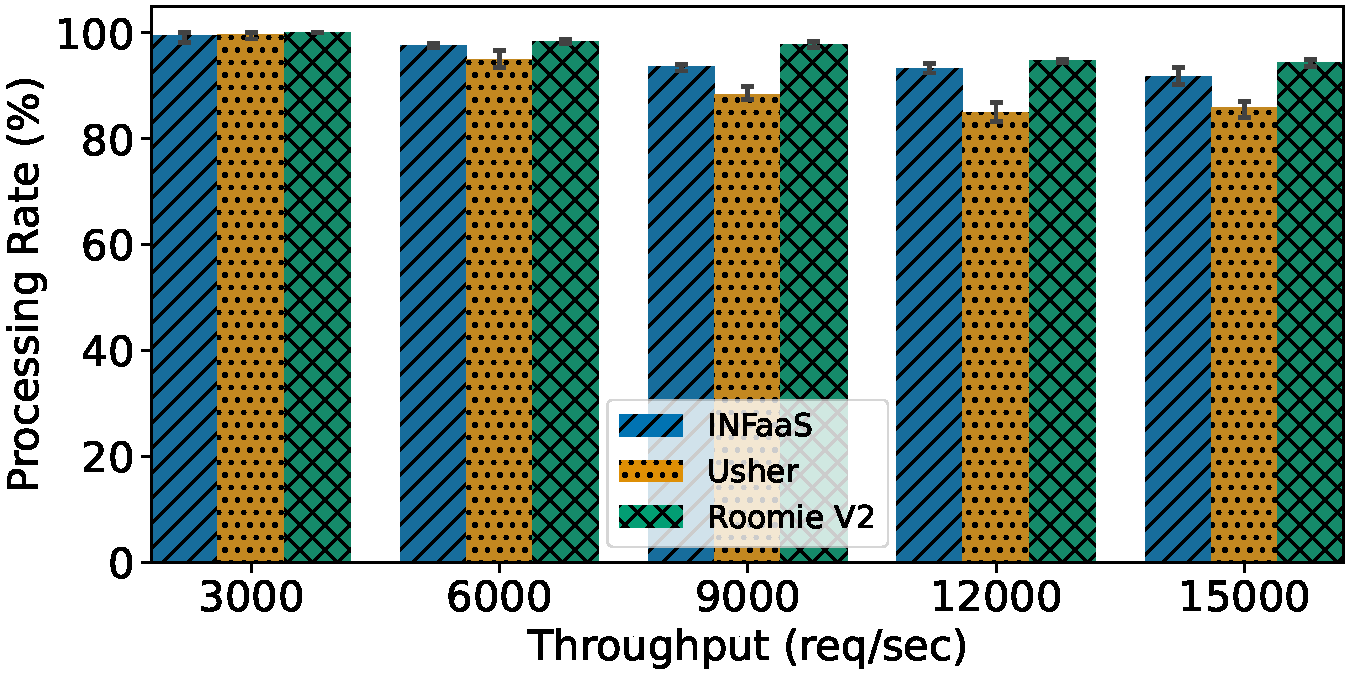
\includegraphics[width=\textwidth]{chapters/roomie/images/NvidiaA100/synthetic-all-models/normalized.pdf}
		\subcaption{Processing rate.}
	\end{subfigure}
	
	\vspace{0.5cm} % Space between the rows
	
	\begin{subfigure}[b]{0.45\textwidth}
		\centering
		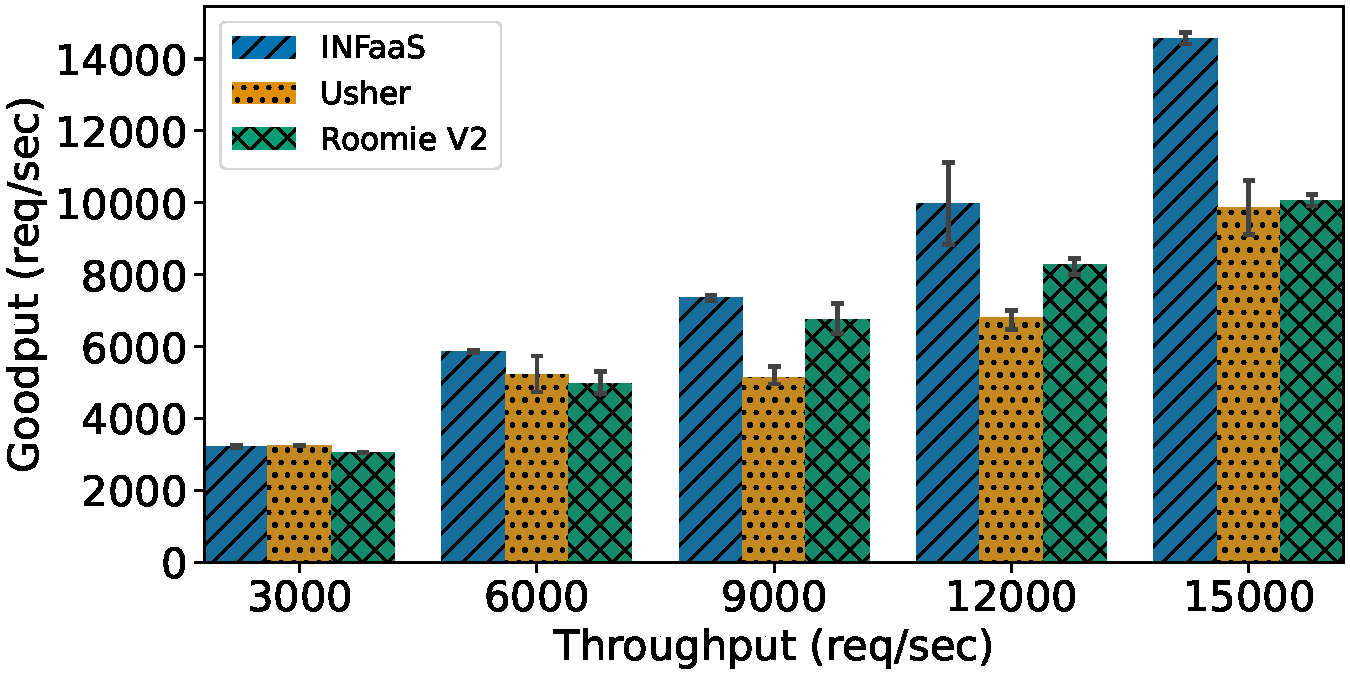
\includegraphics[width=\textwidth]{chapters/roomie/images/NvidiaA100/synthetic-all-models/goodput.pdf}
		\subcaption{Goodput.}
	\end{subfigure}
	\hfill
	\begin{subfigure}[b]{0.45\textwidth}
		\centering
		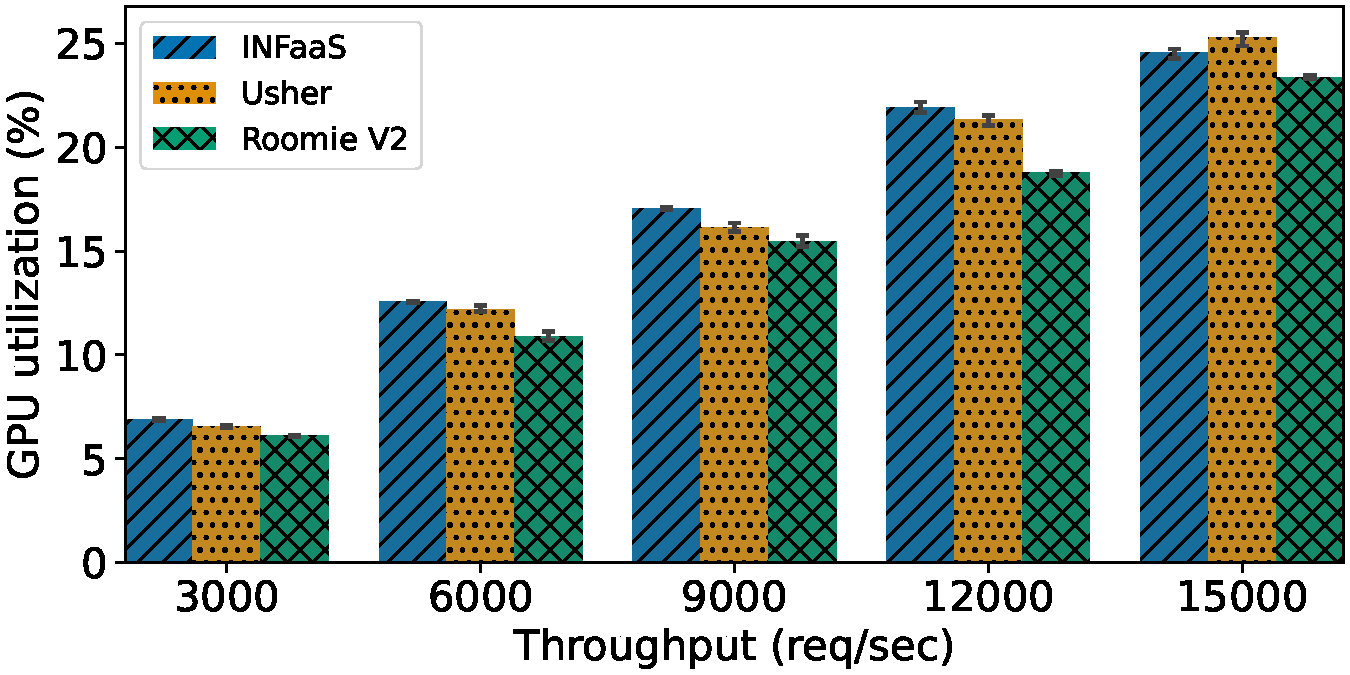
\includegraphics[width=\textwidth]{chapters/roomie/images/NvidiaA100/synthetic-all-models/gpu_utilization.pdf}
		\subcaption{\acrshort{gpu} utilization.}
	\end{subfigure}
	\caption{In cloud-based evaluation using synthetic workloads,~\roomie{} yields 9.2× faster response time and higher processing rate, confirming its deployment efficiency in controlled stress scenarios.}
	\label{fig:NvidiaA100/synthetic-all-models}
	\vspace{-3mm}
\end{figure}


\Cref{fig:NvidiaA100/synthetic-all-models/response-time} illustrates the results of the evaluation conducted with a synthetic dataset designed to emulate diverse and controlled workload scenarios.\\
The performance trends observed with the synthetic dataset closely mirrored those seen with the Twitter data.~\roomie{} consistently outperformed other deployment strategies, achieving a 9.2× reduction in response time and superior throughput and processing rates. These gains are attributed to~\roomie's intelligent model deployment and colocation strategy, which minimizes interference and maximizes resource efficiency.

Overall, across both datasets,~\roomie{} demonstrated robust performance under varying workload conditions. It consistently achieved lower response times—up to 17× faster, and higher processing rate than competing approaches, validating its effectiveness in cloud-based \acrshort{gpu} environments.



\subsection{Performance Evaluation on Edge Devices Using Jetson Xavier \acrshort{gpu}s}

To further validate our approach, we conducted a second set of experiments using a cluster of 12 Jetson Xavier \acrshort{gpu}s, representative of resource-constrained edge computing environments. As in the cloud-based evaluation, we deployed 12 models (from~\Cref{tab:dnn-models}) and tested performance using Twitter data and synthetic data, gradually increasing the workload intensity.

\paragraph{Evaluation on twitter dataset.}

\begin{figure}[h!]
	\centering
	\begin{subfigure}[b]{0.45\textwidth}
		\centering
		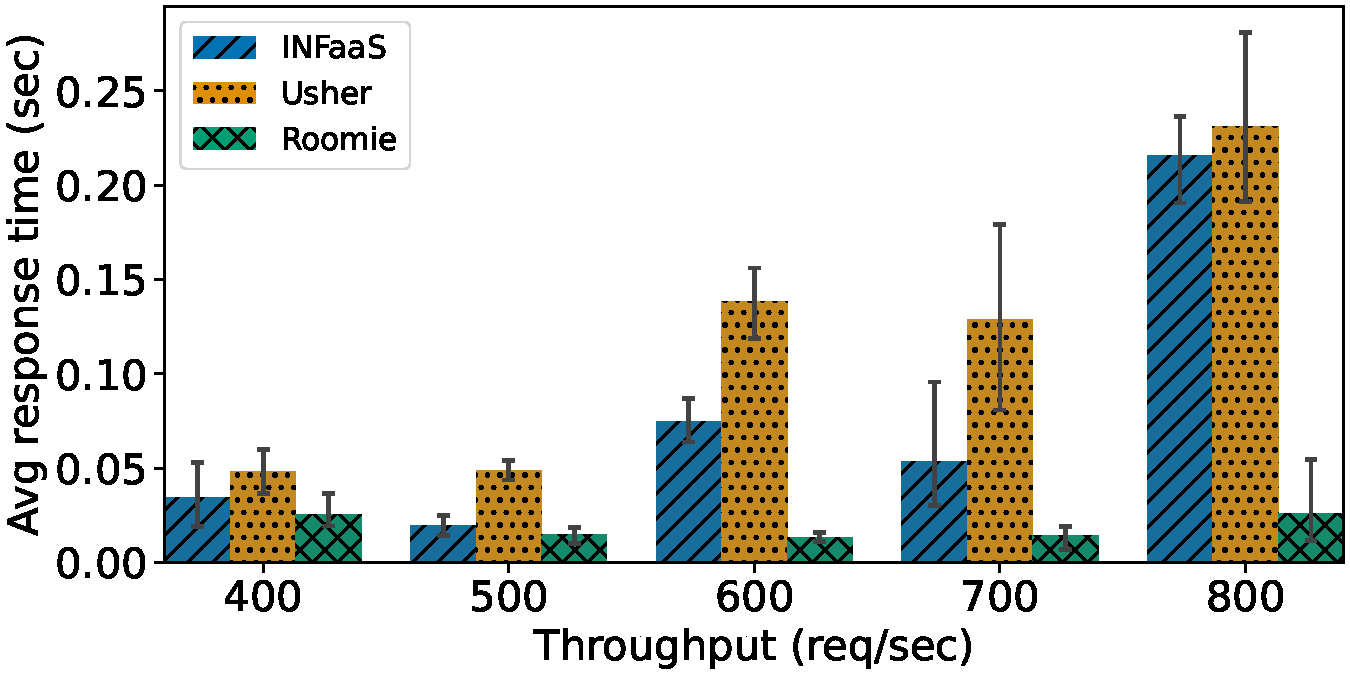
\includegraphics[width=\textwidth]{chapters/roomie/images/JetsonNano/twitter-all-models/response_time.pdf}
		\subcaption{Response time.}
	\end{subfigure}
	\hfill
	\begin{subfigure}[b]{0.45\textwidth}
		\centering
		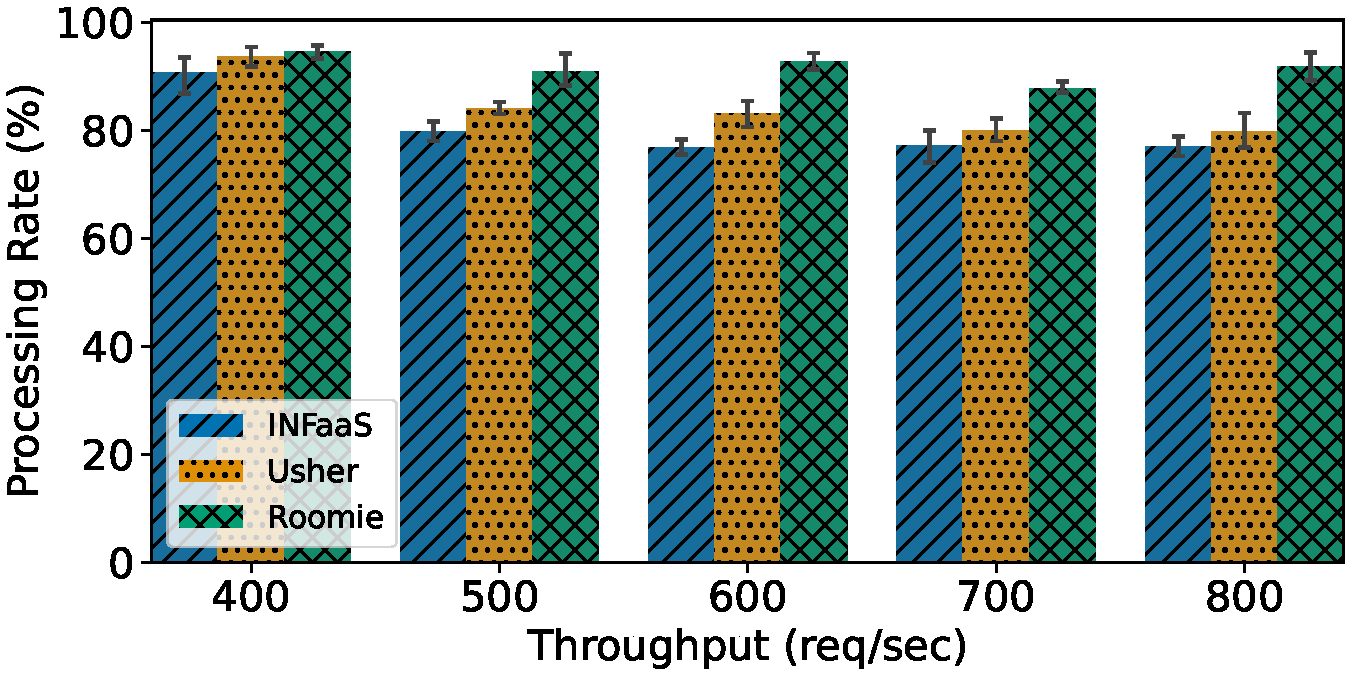
\includegraphics[width=\textwidth]{chapters/roomie/images/JetsonNano/twitter-all-models/normalized.pdf}
		\subcaption{Processing rate.}
	\end{subfigure}
	
	\vspace{0.5cm} % Space between the rows
	
	\begin{subfigure}[b]{0.45\textwidth}
		\centering
		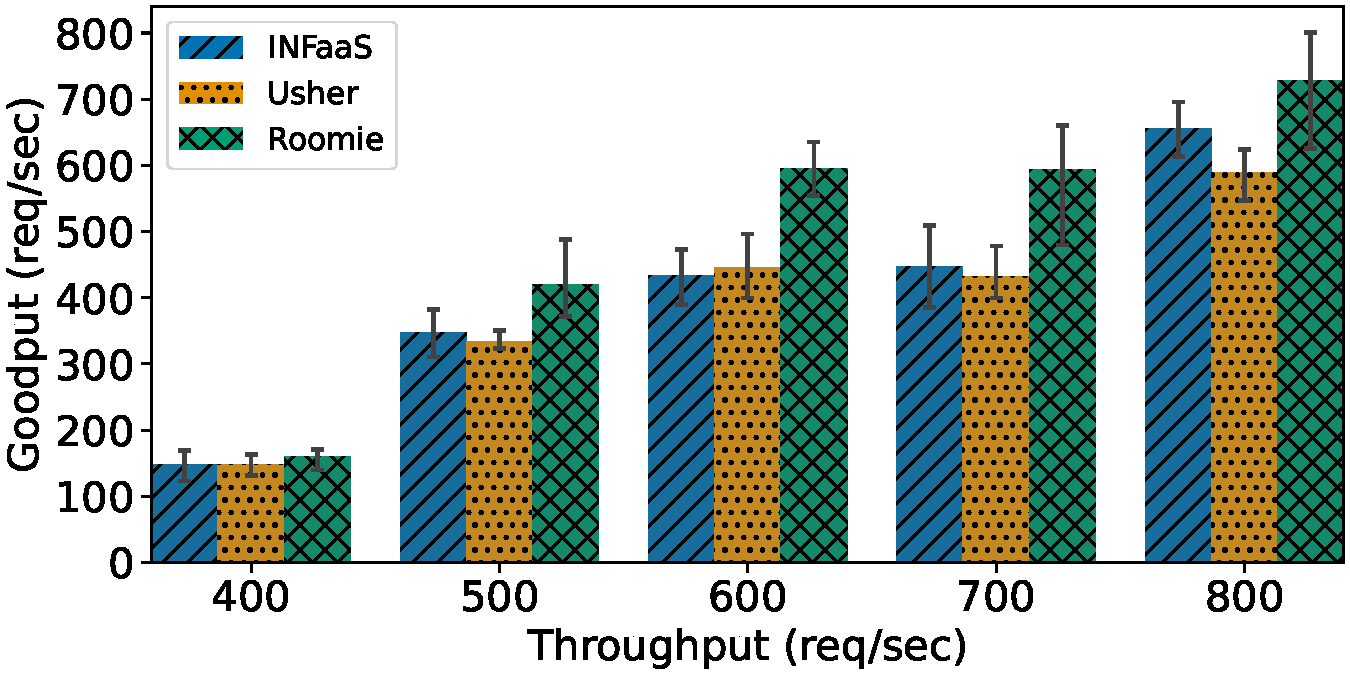
\includegraphics[width=\textwidth]{chapters/roomie/images/JetsonNano/twitter-all-models/goodput.pdf}
		\subcaption{Goodput.}
	\end{subfigure}
	\hfill
	\begin{subfigure}[b]{0.45\textwidth}
		\centering
		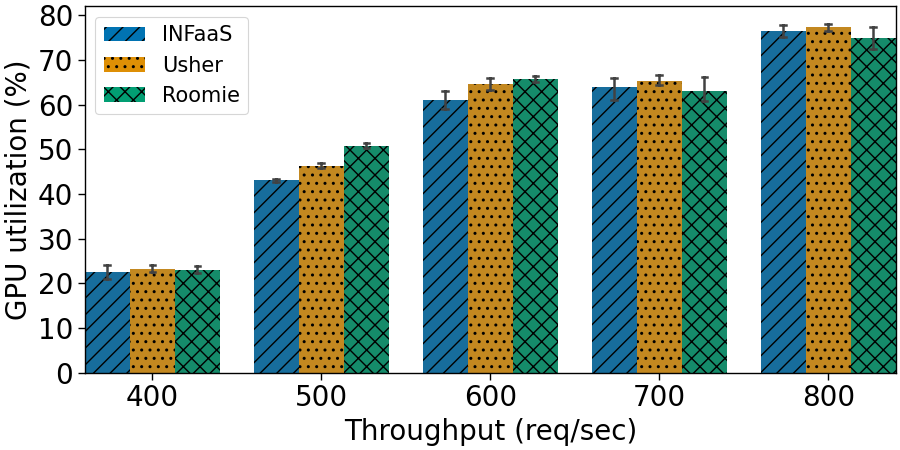
\includegraphics[width=\textwidth]{chapters/roomie/images/JetsonNano/twitter-all-models/gpu_utilization.png}
		\subcaption{\acrshort{gpu} utilization.}
	\end{subfigure}
	\caption{Edge-based evaluation on the Twitter dataset shows~\roomie{} delivering 8.3× lower latency and superior throughput on Jetson Xavier \acrshort{gpu}s, validating its proactive colocation strategy under constrained resources.}
	\label{fig:JetsonNano/twitter-all-models}
	\vspace{-3mm}
\end{figure}

The~\Cref{fig:JetsonNano/twitter-all-models} presents the results obtained with the Twitter dataset on Jetson Xavier devices. While Usher and INFaaS exhibited similar throughput levels, INFaaS achieved lower latency, whereas Usher maintained a higher processing rate.~\roomie, nevertheless, significantly outperformed both, achieving an 8.3× reduction in latency compared to INFaaS under high workload conditions. It also delivered superior throughput and processing rates due to its proactive colocation strategy.

Edge environments impose more severe constraints on model deployment due to limited computing resources and reduced scalability. In this context,~\roomie's colocation strategy offers a significant advantage, effectively balancing resource allocation and minimizing performance degradation. As workload intensity increases, \acrshort{gpu} utilization increases accordingly, reaching levels significantly higher than those seen in cloud-based configurations. This underscores the critical importance of intelligent colocation policies in edge scenarios, where resource efficiency has a direct impact on system responsiveness and throughput.

\paragraph{Evaluation on synthetic dataset.}

\begin{figure}[h!]
	\centering
	\begin{subfigure}[b]{0.45\textwidth}
		\centering
		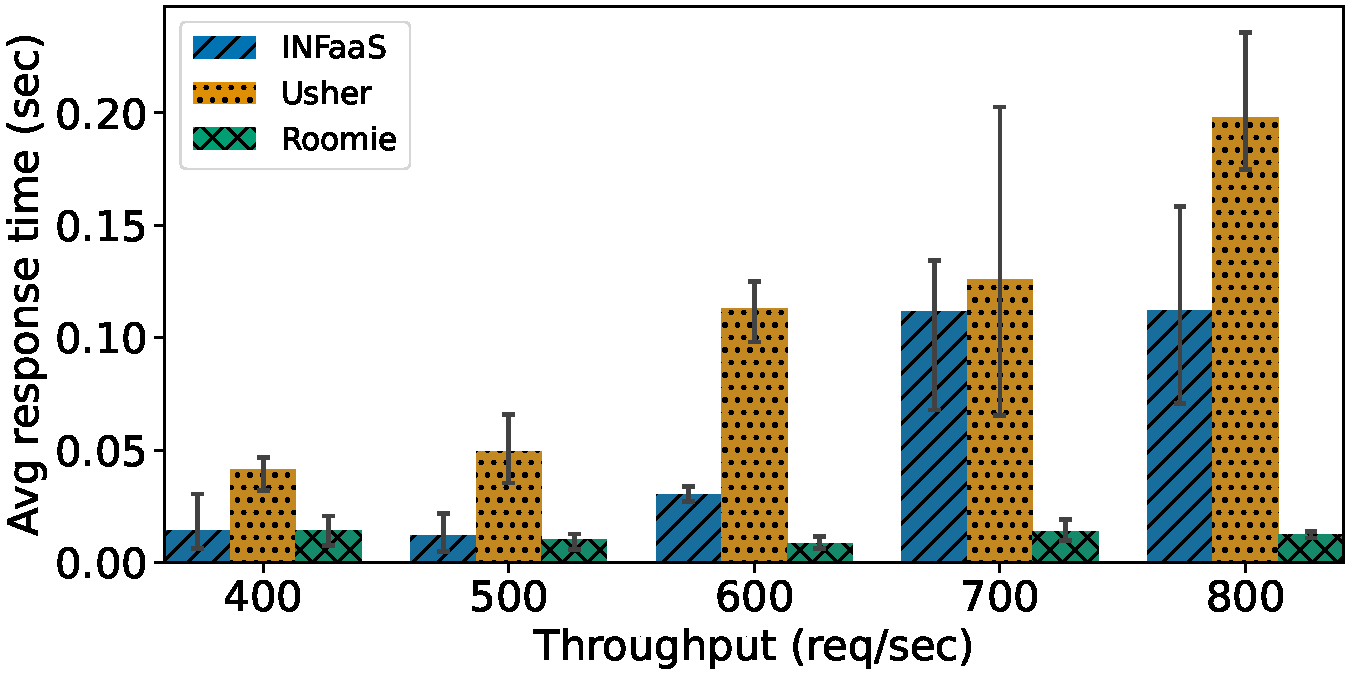
\includegraphics[width=\textwidth]{chapters/roomie/images/JetsonNano/synthetic-all-models/response_time.pdf}
		\subcaption{Response time.}
	\end{subfigure}
	\hfill
	\begin{subfigure}[b]{0.45\textwidth}
		\centering
		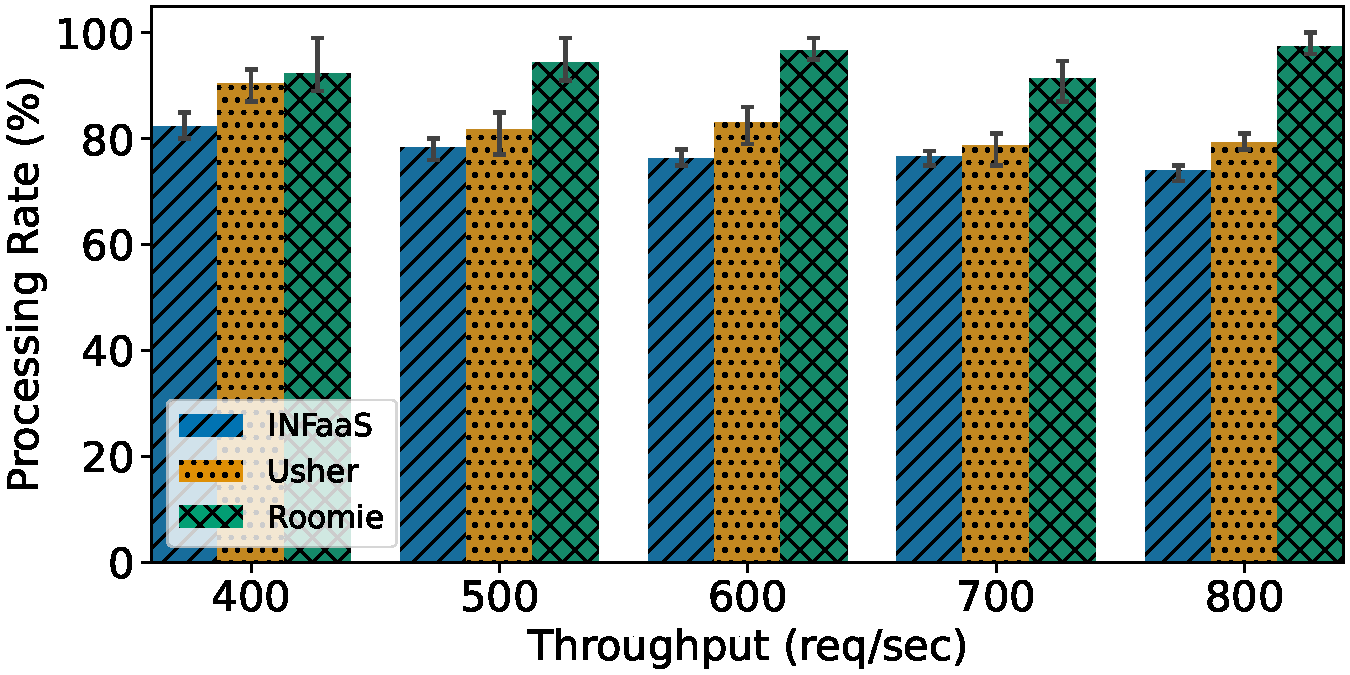
\includegraphics[width=\textwidth]{chapters/roomie/images/JetsonNano/synthetic-all-models/normalized.pdf}
		\subcaption{Processing rate.}
	\end{subfigure}
	
	\vspace{0.5cm} % Space between the rows
	
	\begin{subfigure}[b]{0.45\textwidth}
		\centering
		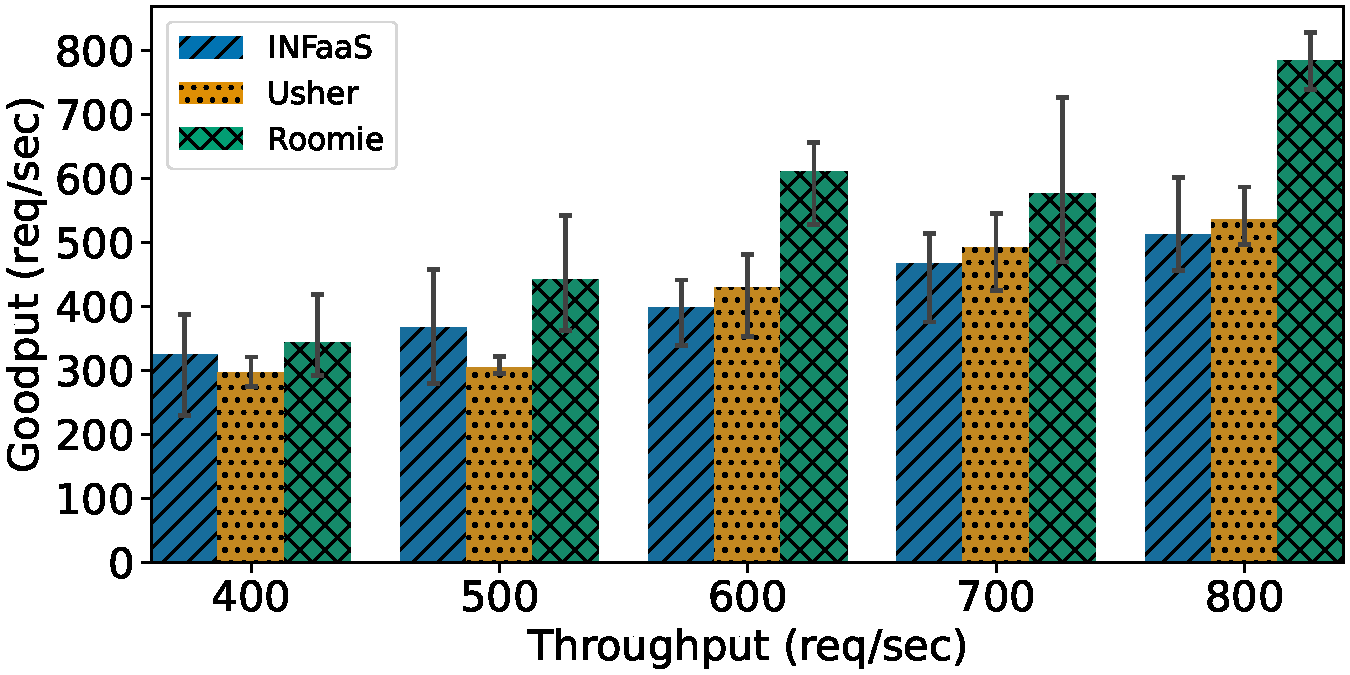
\includegraphics[width=\textwidth]{chapters/roomie/images/JetsonNano/synthetic-all-models/goodput.pdf}
		\subcaption{Goodput.}
	\end{subfigure}
	\hfill
	\begin{subfigure}[b]{0.45\textwidth}
		\centering
		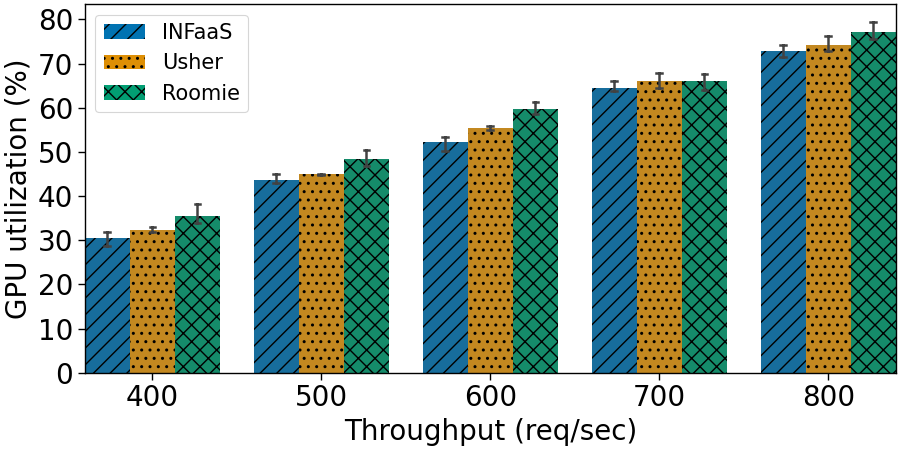
\includegraphics[width=\textwidth]{chapters/roomie/images/JetsonNano/synthetic-all-models/gpu_utilization.png}
		\subcaption{\acrshort{gpu} utilization.}
	\end{subfigure}
	\caption{Under synthetic edge evaluation,~\roomie{} sustains 9× faster response time and 1.5× higher throughput, demonstrating robust performance in resource-limited environments.}
	\label{fig:JetsonNano/synthetic-all-models}
	\vspace{-3mm}
\end{figure}

The synthetic dataset evaluation on Jetson Xavier \acrshort{gpu}s yielded consistent results with those observed on the Twitter dataset. The results are shown in~\Cref{fig:JetsonNano/synthetic-all-models}.~\roomie{} again demonstrated superior performance, achieving a 9× reduction in response time and a 1.3× increase in processing rate. Throughput was also 1.5× higher than competing approaches.

These findings confirm that~\roomie{} is the most effective \acrshort{dnn} deployment strategy in edge computing contexts where colocation is necessary and resources are limited. Its ability to maintain low latency and high throughput under constrained conditions makes it a compelling solution for real-time inference workloads.


\subsection{Evaluating~\roomie{} Deployment Accuracy Against Optimal Strategies}

\begin{figure}[t!]
	\centering
	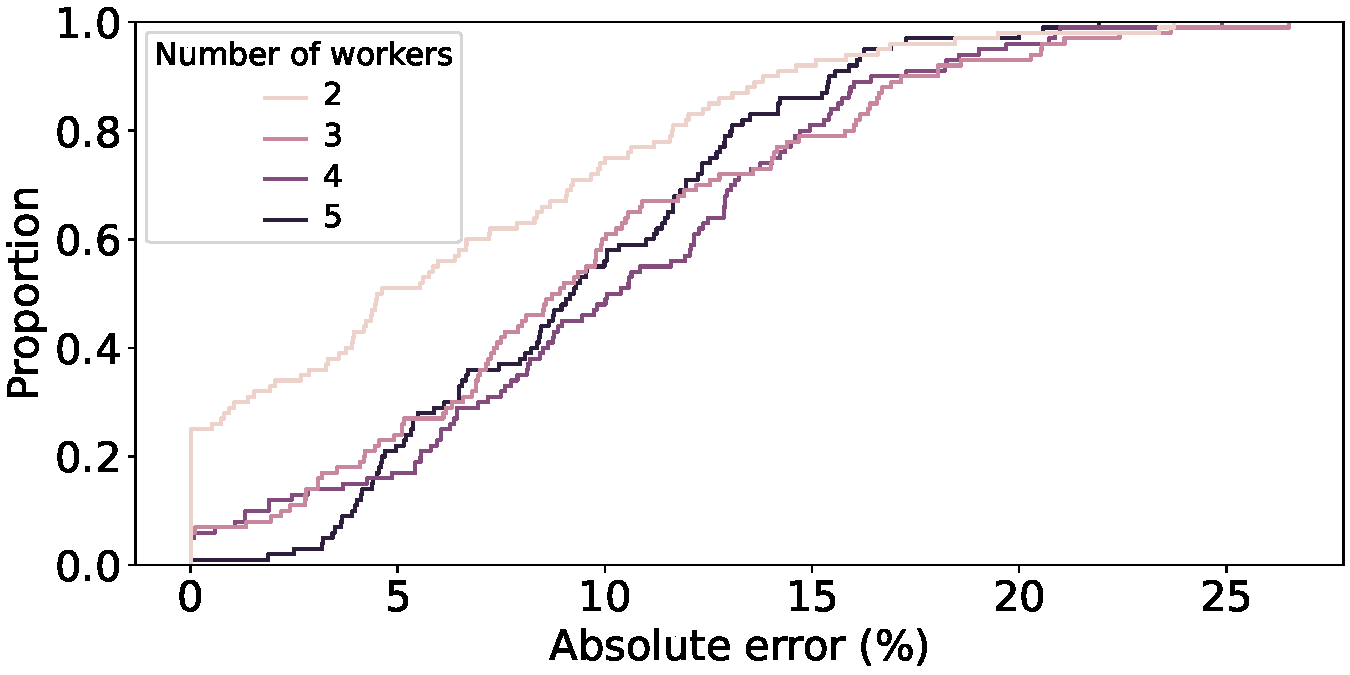
\includegraphics[width=\textwidth]{chapters/roomie/images/performance_gap_per_worker.pdf}
	\caption{Empirical CDF of~\roomie's performance gap relative to the optimal deployment strategy.}
	\label{fig:performance_gap}
\end{figure}

This section investigates the efficacy of~\roomie{} for the deployment of \acrshort{dnn}s across a varying number of workers, specifically between two and five. For each configuration, the quantity of \acrshort{dnn}s to be deployed was randomly selected from a range of two to three times the number of workers, guided by predefined options outlined in~\Cref{tab:dnn-models}. More than 100 randomized evaluations were conducted to ensure comprehensive coverage of deployment scenarios. In each evaluation, all feasible deployment permutations were thoroughly assessed to determine the configuration that resulted in the minimal average performance drop, defined as the optimal baseline. Subsequently, \roomie{} approach was applied to the same scenarios, and the absolute error between \roomie{} and optimal deployments was calculated. The cumulative distribution function (CDF) in~\Cref{fig:performance_gap} summarizes the accuracy of~\roomie{} deployment strategy for deep neural networks (\acrshort{dnn}s).

The first key observation lies in the low-error range. With two workers, 25\% of deployments fall below 0.4\% error, indicating that~\roomie{} often achieves near-optimal results in simple configurations. This sharply contrasts with higher concurrency levels, where the lower quartile rises to over 5\% for three or more workers. This shift reflects the increasing difficulty of estimating performance under competitive conditions, where profiling tools such as Nsight-Compute introduce overhead that distorts kernel execution metrics central to the modeling process.\\
The second key value is the central tendency. The median error climbs from 4\% with two workers to 10\% with four, before slightly receding with five. This peak coincides with the most pronounced modeling challenges, where pairwise colocation and reduced configuration space, used to accelerate convergence, begin to weaken. As concurrency increases,~\roomie{} must account for overlapping execution schedules and interleaved kernels, which obscure the relative timing of model completions and complicate inference behavior.\\
Third, the highest observed errors across configurations do not follow a consistent upward or downward trend, but instead fluctuate with concurrency. It rises from 13\% with two workers to 17\% with three, then drops slightly to 16\% with four and further to 15\% with five. This pattern suggests that while~\roomie{} faces its greatest challenges in intermediate configurations, it regains robustness as the system becomes more distributed. The added flexibility at higher concurrency levels appears to mitigate some of the estimation noise introduced by profiling and architectural interference.

Overall, the analysis demonstrates that~\roomie{} performs reliably under low concurrency and remains competitive even as complexity increases. Its ability to maintain bounded error across a wide range of deployment scenarios is particularly notable given the inherent challenges of performance estimation in \acrshort{gpu} environments. Profiling remains indispensable for capturing fine-grained kernel behavior, despite its overhead and distortion effects.~\roomie's design, grounded in practical strategies such as pairwise colocation and reduced configuration space, proves effective in navigating these constraints. While intermediate concurrency levels expose the limits of current modeling techniques, the overall performance remains within acceptable bounds, validating~\roomie{} as a scalable and interference-aware solution for multi-model deployment.
\label{lastpage}\section{Conclusion}\label{sec:conclusion}

\roomie{} consistently delivers high-performance deployments across both cloud and edge \acrshort{gpu} environments. In cloud settings, it achieves up to 17× lower latency and maintains over 97\% processing rate, outperforming competing strategies through interference-aware colocation and saturation resilience. On edge devices,~\roomie{} sustains its advantage with up to 9× lower response times and 1.5× higher throughput, effectively navigating resource constraints. Its heuristic maintains bounded error relative to the optimal deployment, often within 10\% even under high concurrency, despite challenges such as profiling overhead and architectural variability. These results hold across real-world and synthetic datasets, confirming~\roomie{}'s robustness and scalability. By intelligently minimizing cross-model interference and adapting to resource constraints,~\roomie{} proves to be a practical and interference-aware solution for multi-model inference in modern \acrshort{gpu} systems.
